\documentclass[12pt]{article}
\usepackage{amsmath, amssymb, amsfonts}
\usepackage[margin=1in]{geometry}
\usepackage{setspace}
\usepackage{parskip}
\usepackage{fancyhdr}
\usepackage{graphicx}
\usepackage{subcaption}

\pagenumbering{arabic}
\linespread{1.5}
\setlength{\parskip}{12pt}
\pagestyle{fancy}
\fancyhf{}

\lhead{Ningrui Xie}
\chead{BIO 4C12 Midyear Report}
\rhead{ID: 400323416}
\fancyfoot[C]{\thepage}
\renewcommand{\headrulewidth}{0pt}
\newcommand{\perday}{\ensuremath{\mathrm{/day}}}

\begin{document}


\title{Mathematical Approaches for Simulating Epidemic Progression: Addressing Limitations of the Linear Chain Trick in ODE Models}

\author{Submitted to\\ Dr. Jonathan Dushoff 
\\McMaster University\\Hamiltion, Ontario, Canada L8S 4K1}
\date {January 1, 2024}
\maketitle


\centerline{Reported by}
\centerline{\textbf{Ningrui Xie}}
\centerline{\textbf{400323416}}


\newpage
\section{Abstract}
The SIR framework, because of its simplicity and ability to describe dynamic changes, is widely used in infectious disease modeling. One issue with the traditional SIR model is its implicit assumption of an exponentially distributed infectious stage duration, which often diverges from real-world scenarios. A common solution is the application of the Linear Chain Trick (LCT), wherein the single infectious stage is divided into several substages, each following an exponential distribution. The incorporation of LCT results in an Erlang distributed stage duration. However, despite its widespread application, LCT presents challenges, including the complex determination of substage numbers and rigid parameter values. Here, we propose a novel approach, maintaining a fixed number of substages but employing a geometrically distributed substage transition rate. This method, while akin to LCT in its foundational principles, offers greater flexibility in defining the stage duration shape. In contrast to the recently introduced Generalized Linear Chain Trick (GLCT), which broadens the scope to encompass a wider range of phase-type distributions, our method provides a more straightforward and efficient means to achieve model flexibility. Although our discussion focuses on epidemic modeling, the potential applications of this approach extend to various forms of dynamic modeling, offering advantages in terms of computational efficiency, ease of parameter estimation, and adaptability to diverse modeling scenarios. 


\section{Introduction}
Ordinary differential equations (ODEs) are a popular choice for mathematical modeling in biology due to their ability to accurately represent the dynamic processes of systems over time. ODEs provide a powerful framework for describing phenomena such as population dynamics \cite{salisbury2011mathematical}\cite{sego2021generation}, the spread of infectious diseases \cite{Anderson1991}\cite{Diekmann2000}\cite{Feng2016}, and cell proliferation (e.g., cancer) \cite{baker1998modelling}\cite{jarrett2018mathematical}, which are characterized by continuous state changes. The inherent flexibility and simplicity of ODEs make them not only easy to solve and understand but also easy to manipulate and accommodate to various situations.

In the field of epidemiology, ordinary differential equations (ODEs) serve as a powerful tool to characterize the progression of diseases and to make predictions. A commonly used model is the SIR compartmental model \cite{Anderson1991}\cite{kermack1927contribution}, which divides the population into three states: Susceptible, Infectious, and Recovered. In this model, a susceptible individual, upon contact with the infected population at a rate $\beta$, transitions immediately to the infectious state. An infected individual then moves to the recovered state at a recovery rate of $\gamma$. However, one major limitation of this model is its implicit assumption that the duration of the infectious stage follows an exponential distribution. This can be seen in a simplified equation modeling the dynamics of the infected population

JD: This is what I mean by the cohort equation (see below). Also, probably it's good to have more numbered equations and fewer anonymous ones like this.
\begin{align*}
    \frac{dI}{dt} = -\gamma I
\end{align*}
Solving this equation explicitly yields
\begin{align*}
    I(t) = I_0 e^{-\gamma t}
\end{align*}
which implies a stochastic state transition model where the time spent in the infectious stage $I$ is exponentially distributed with a mean stage duration of $\frac{1}{\gamma}$. This dwell time distribution suggests that an individual is most likely to recover immediately after infection, which is often not realistic. In reality, a delay between the successful infection of an individual and the recovery from the disease is inevitable, as shown in studies conducted by Greenhalgh and Day (2017) \cite{greenhalgh2017time} using measles outbreak data. JD: “inevitable” does not match well with “shown”.

The constraint of the basic ODE framework is that it primarily offers a singular approach to assuming specific dwell time distributions: the first event time distribution of a nonhomogeneous Poisson process, including the exponential distribution as a special case \cite{hurtado2019generalizations}. This inflexibility in specifying probability distributions to describe the duration individuals spend in a given state is a nonnegligible shortcoming of the SIR model. JD: This seems to be going too deep; the “basic” ODE framework is assuming exponential.

It is important to note that even when the mean is constant, the shape of the stage duration distributions (i.e., the timing of stage transitions) can significantly impact the dynamics and the outcomes of predictive models in applied settings \cite{krylova2013effects}\cite{keeling2002understanding}\cite{wearing2005appropriate}\cite{nguyen2008noise}. Consequently, it becomes crucial to consider the type of distribution characterizing an individual in a specific state when constructing these models. A standard approach for developing models that incorporate different stage duration distributions is through the use of integro-differential equations (IDEs) or integral equations (IEs) \cite{hurtado2019generalizations}\cite{kermack1927contribution}\cite{hethcote1980integral}. IDEs facilitate the extension of the SIR model to include arbitrary distributions for the duration of infectiousness, as discussed in various sources \cite{feng2000endemic}\cite{hethcote1980integral}\cite{ma2006generality}. This approach allows for the capture of the 'memory effect', where the current rate of change in each compartment of the model (Susceptible, Infectious, Recovered) is influenced by the entire history of the epidemic, rather than relying on a constant rate assumption.

However, while integro-differential equations enhance the model's flexibility, they are often challenging to formulate, analyze mathematically, and simulate, especially when compared to ordinary differential equations \cite{krylova2013effects}\cite{hurtado2019generalizations}\cite{burton2005volterra}. There have been efforts to simplify IDEs into systems of ODEs \cite{macdonald2008biological}\cite{ponosov2004thew}\cite{burton2005volterra}\cite{goltser2013reducing}\cite{diekmann2018finite}, with the most notable example being the reduction of IDEs that assume Erlang-distributed stage durations \cite{hurtado2019generalizations}. Unlike the exponential distribution, a more biologically plausible assumption might be a probability distribution where the likelihood of exiting the infectious stage starts small, increases as it nears the mean duration of infection, and eventually diminishes to zero as time extends indefinitely \cite{sartwell1966incubation}\cite{bailey1954statistical}. Due to its central tendency towards the mean value, the Erlang distribution, defined as a gamma distribution with an integer shape parameter, is a more realistic choice for depicting the duration of the infectious stage. The integration of the Erlang distribution into the ODE system is facilitated by the Linear Chain Trick (LCT) \cite{macdonald1978time}\cite{smith2011introduction}. In this approach, the single infected state is divided into $n$ substages, each following an exponential distribution with a rate of $n\gamma$. This technique is based on the principle that the sum of a series of independent exponentially distributed random variables follows a gamma distribution \cite{krylova2013effects}\cite{therrien2018probability}. When the LCT is applied to the SIR model, the number of substages $n$ determines the shape of the stage duration distribution. As $n$ increases, the variance decreases, resulting in a distribution that is more peaked and narrow around the mean value $\frac{1}{\gamma}$. As $n$ approaches infinity, the distribution converges to a delta function (a deterministic value, implying that all individuals who become infectious at time $t$ recover at exactly time $t + \frac{1}{\gamma}$), and the system evolves into a delay differential equation \cite{krylova2013effects}\cite{hethcote1980integral}.
JD: This \P\ is very long and doesn't really explain well the key point. I might explain in the other direction: LCT equations are much simpler than IDEs, and can produce dwell distributions that are more realistic than the basic model. The fact that the the n-box LCT formulation is an Erlang is kind of a detail.

The Linear Chain Trick (LCT) is extensively employed in modeling biological processes, not only in quantifying disease progression \cite{lloyd2001destabilization}\cite{lloyd2001realistic}, but also in analyzing virus \cite{lloyd2001dependence}\cite{kakizoe2015method} and population \cite{cushing2013integrodifferential} dynamics. Studies have demonstrated that switching the stage duration distribution from an exponential to an Erlang distribution leads to predictions that align more closely with real data points \cite{kakizoe2015method}. However, despite the increased realism they bring to modeling disease processes, employing LCT in ODE models presents several limitations. One primary challenge is determining the appropriate number of substages $n$ to divide, which is a cumbersome and time-consuming process. Multiple models with varying substages must be constructed and subjected to repeated data-fitting processes to identify the optimized parameter value. Prior research has investigated approaches for estimating the number of states in the linear chain, employing techniques such as profile likelihood \cite{raue2009structural} and model reduction \cite{maiwald2016driving}. Yet, a comparative study of these methods indicates that the typical quality of experimental data is insufficient for reliably estimating the chain length using these approaches \cite{hauber2020estimating}. Another inherent limitation of using LCT is the inflexibility of the model's parameters. To integrate $n$ independent exponentially distributed random variables into the ODE system, $n$ must be an integer. As the subdivision process is done without altering the overall mean of the stage, the rate of each substage $n\gamma$ is also constrained to discrete values. These limitations significantly restrict the adaptability and practical application performance of the model.

The recently proposed Generalized Linear Chain Trick (GLCT) enhances the Linear Chain Trick (LCT) by enabling models to incorporate a broader phase-type family of distributions \cite{hurtado2019generalizations}\cite{hurtado2021building}\cite{bladt2017phase}, which includes exponential, Erlang, hypoexponential, and Coxian distributions, thus allowing for greater flexibility and the ability to capture more complexity. The GLCT achieves this by creating a higher-dimensional Markov chain, enabling a more accurate representation of the complex nature of dwell time distributions. However, this process can be mathematically heavy and challenging to interpret. Additionally, this approach may lead to a increase in the number of variables or states within the model, potentially escalating computational demands. Therefore, finding a simpler and more efficient method to enhance the flexibility of the ODE model remains essential.

In this study, we focused on one particular direction: generalizing the Erlang distribution of stage durations currently present in the model. The goal was to allow for a more diverse range of shapes, achieved by eliminating the constraints imposed by the shape parameter ($\kappa$). The value of $\kappa$ in the SInR model was limited to a set of discrete values, as detailed below. To address this limitation, as well as those previously mentioned, we propose a novel approach. Instead of using a variable number of substages $(n)$ with a constant rate $(\gamma_i = n\gamma)$ for all exponentially distributed substages, we fix $n$ to a specific integer value and use a series of rates that follow a geometric pattern. This series is represented by the formula $\gamma_i = ar^{i-1}$, governed by parameters $a$ and $r$. Consequently, the parameter of interest shifts from discrete values $(n$ and $ng)$ to continuous values $(a$ and $r)$, thereby enhancing the model's adaptability.

To illustrate this point, consider that the Gamma distribution can be parameterized in terms of its mean $(M)$ and shape parameter (quadratic coefficient of variation, $\kappa$), which determine the overall shape and position of the distribution. As mentioned above, in subdividing a single stage into n substages, each exponentially distributed substage must have a rate of $n\gamma$ to maintain the overall rate of that stage. While the mean of the Erlang distribution in the ODE system can be chosen freely, $\kappa$ is constrained to discrete values, shown as follows:
\begin{align*}
    Mean: \quad &\sum_{i=1}^{n_f} \frac{1}{n\gamma} = \frac{1}{\gamma}\\
    Variance: \quad &\sum_{i=1}^{n_f} \frac{1}{n^2\gamma^2} = \frac{1}{n\gamma^2} \\
    \kappa: \quad &\frac{\sigma^2}{M^2} = \frac{1}{n} \quad n \in \mathbb{N}
\end{align*}
Our approach, using a geometric series of rates, addresses this issue by allowing $\kappa$ to take any value within the range $[\frac{1}{n}, 1)$. A detailed explanation and the derivation process are provided in section $4.2$. Another advantage of this method is that it enables a fixed model structure where only the parameters change, eliminating the need to determine optimal substage numbers through the construction of multiple models, a process currently required in the ODE model that employs the LCT.

Throughout this research, we primarily focused on the application of the LCT in the epidemic SIR model, which we refer to as the SI$^n$R model, where $n$ represents the number of substages divided. The objective of our study is to develop and evaluate the method of using a geometrically distributed substage rate as a replacement for the constant rate, aiming to enhance flexibility and efficiency. We have named the model that utilizes this method the SIgR model (temporarily). We anticipate that this approach will not only be computationally efficient but also provide a better fit to real-world data. In the following sections, we first aim to align the infectious stage duration distribution shapes generated by the SI$^n$R and SIgR models. Once we have confirmed that our proposed model can effectively substitute the SInR model, we proceed to allow the SIgR model to include stage duration distributions with characteristics unattainable by the SI$^n$R model. We then invert the process: given a desired mean and $\kappa$, we develop the computational system to determine the parameter values $(a$ and $r)$ that enable the model to produce a stage duration distribution with these properties. Subsequently, we will conduct empirical validation of our model through data fitting. This evaluation will cover aspects such as the model’s consistency with dataset and its predictive accuracy in forecasting future trends. We predict that this approach will enhance the model’s adaptability and practicality, thus paving the way for the development of user-friendly software tools that empower modelers to efficiently select and employ the most suitable models for describing and predicting future epidemic scenarios.



\section{Method}
Several assumptions have been made for the unforced SIR model (Susceptible, Infectious, and Recovered) that our study is based on: 
\begin{enumerate}
    \item \textbf{Closed Population}: A constant population size with equal birth and death rates and no disease-related mortalities.
    \item \textbf{Homogeneous mixing}: Individuals have an equal chance of coming into contact with any other individual in the population. 
    \item \textbf{Ignoring Latency}: Individuals move immediately from a susceptible state to an infected state, ignoring any incubation period associated with the disease.
    \item \textbf{Lifelong immunity}: Once an individual recovers, they do not become susceptible or infectious again.
\end{enumerate}
We also assume that the state variables have been scaled by the total population size $N$ so that $S + I + R = 1$. The SIR model can be expressed as a simple system of nonlinear ordinary differential equations:
\begin{align}
    \frac{dS}{dt} &= \mu - \beta SI - \mu S \\
    \frac{dI}{dt} &= \beta SI - \gamma I - \mu I \\
    \frac{dR}{dt} &= \gamma I - \mu R
\end{align}
where $\mu$ is the birth and natural mortality rate, $\beta$ is the disease transmission rate, and $\gamma$ is the recovery rate. The mean recovery time for an infected individual is $\frac{1}{\gamma}$. 

The idea of dividing the infectious stage into $n$ sub-stages exploits the fact that the sum of a sequence of independent, exponentially distributed random variables follows an Erlang distribution (i.e. gamma distributed with integer shape parameter) \cite{therrien2018probability}. Thus, we begin by confirming the uniformity of the results generated by simulating the SI$^n$R model with the Erlang distribution, which has the following form:
\begin{equation*}
    f(x; n,n\gamma) = \frac{(n\gamma)^n}{(n-1)!} x^{n-1} e^{-n\gamma x} \quad x>0, n \in \mathbb{N}
\end{equation*}

By breaking a single stage into $n$ substages, each exponentially distributed with a rate of $n\gamma$ ($\gamma_i = n\gamma$), the SI$^n$R model can be represented by a system of ODEs:
\begin{align*}
    \frac{dS}{dt} &= \mu - \beta SI - \mu S \\
    \frac{dI_1}{dt} &= \beta SI - (n \gamma + \mu) I_1 \\
    \frac{dI_2}{dt} &= n\gamma I_1 - (n \gamma + \mu) I_2 \\
    &\vdots \\
    \frac{dI_n}{dt} &= n\gamma I_{n-1} - (n \gamma + \mu) I_n \\
    \frac{dR}{dt} &= n \gamma I_n - \mu R
\end{align*}

Note that this decomposition process will not change the mean stage duration, as the sum of the means of the $n$ exponentially distributed random variables still equals $\frac{1}{\gamma}$
\begin{align*}
    \frac{1}{\gamma} = \sum_{i=1}^{n} \frac{1}{n\gamma}
\end{align*}

JD: I feel there's some confusion below. When thinking about the cohort model (like the very first displayed equation), we focus on dynamics of recovered. That's how we construct our infectious-period distributions. But when thinking about a transmission model (like the one below), we typically focus on incidence (cumulative, interval and instantaneous). For your thesis, it might be good to explicitly write out cohort models to support the stage-distribution stuff above, and to clarify the distinction between cohort models and transmission models. The reason I call them cohort models is that each “cohort” of 

For consistency, we focused exclusively on the dynamics of the recovered compartment. The simulation results generated by the SI$^n$R model represent the cumulative distribution of the recovered population. Therefore, we need to take the derivative to convert it into a probability density function, allowing for comparison with the Erlang distribution. After confirming that the stage duration distribution generated by the SI$^n$R model aligns with a gamma distribution with an integer shape parameter, we constructed the SIgR model. This model has a fixed number of substages $n_f$ and features substage rate that are geometrically distributed ($\gamma_i = ar^{i-1}$), shown as follow
\begin{align*}
    \frac{dS}{dt} &= \mu - \beta SI - \mu S \\
    \frac{dI_1}{dt} &= \beta SI - (a + \mu) I_1 \\
    \frac{dI_2}{dt} &= a I_1 - (ar + \mu) I_2 \\
    &\vdots \\
    \frac{dI_n}{dt} &= ar^{n-1} I_{n-1} - (ar^n + \mu) I_n \\
    \frac{dR}{dt} &= ar^n I_n - \mu R
\end{align*}

JD: It would be good to have a clearer explanation of the goal. “Effective” is not very explicit here.
We aim to determine if altering the parameter $a$ and $r$ is more effective than changing the number of substages. Our starting point involves keeping the mean stage duration $(M)$ constant while varying $r$ to explore the possibility of a match between the SI$^n$R and SIgR models. This match will be assessed both by the mean $(M)$ and by the shape parameter, which is the coefficient of variation squared $(\kappa = \frac{\sigma^2}{M^2})$.
JD: Not sure why you're using $M$, and whether you really mean the mean “stage” duration. We should be focused on the mean total duration, and call it $D$, I think.

After determining the potential match, we have formulated the formulas for $M$ and $\kappa$ in terms of $a$ and $r$. Utilizing the geometric distribution of rates in the ODE model allows for independent changes in $M$ and $\kappa$. This enables us to achieve the desired value of $\kappa$ without altering the mean, and vice versa. Our goal is to reverse the method: starting with given values of $M$ and $\kappa$, we aim to find specific values of $a$ and $r$ that will let the model generate the stage duration distribution that satisfies these properties. Due to the complexity introduced by the high powers in the formula, solving it explicitly is challenging. To address this, we have developed a system of functions in the R programming language, employing the uniroot() function to obtain a numerical solution for r. We then reintegrate this parameter value into the SIgR model and compare it with the SInR model, using the same $M$ and $\kappa$ values. Subsequently, the mean and the shape parameter of both simulation results are calculated numerically to confirm the validity of the match.

After confirming that the newly proposed model can effectively replace the SI$^n$R model by encompassing the same infectious stage duration distributions, we will proceed to empirically test the enhanced performance of the model through data fitting. This process will be divided into two phases and will be conducted in R using the \textbf{bbmle} package. As the starting point, we will employ a deterministic model and assume only observation noise. Our first step involves coding to generate a `fake' dataset, treating the disease incidence time series from the SIgR model as the actual case, and introducing deviations (noises) into them using a mean reporting ratio and a negative binomial dispersion parameter. The model parameters will then be estimated using the Maximum Likelihood Estimation (MLE) method, applied to the fake dataset. The objective here is to accurately recover the original parameter values that were used to generate the disease incidence data. In the next phase of the study, we will fit the model using an real-world dataset. We plan to compare the fitting results obtained from both the SI$^n$R and SIgR models. This will allow us to quantitatively assess the efficacy of our proposed method in improving the model's accuracy in reflecting actual epidemiological scenarios.




\section{Results}
In Figure 1, we present the comparison plots between the infectious stage duration distribution generated by the SI$^n$R model with the Erlang distribution. In this model, the mean recovery time is set to be 10 days $(\gamma = \frac{1}{10})$ and the infectious stage is divided into $n$ substages $(n = 4, 8, 12, 18)$, with each substage having a rate of $\frac{n}{10}$. The corresponding shape and scale parameters for the gamma distribution are $n$ and $\frac{n}{10\perday}$, respectively. The plot demonstrates a perfect match between the two distributions, despite being generated by different methods. In the subsequent sections, we will refer to these two distributions interchangeably.
\begin{figure}[h]
    \centering
    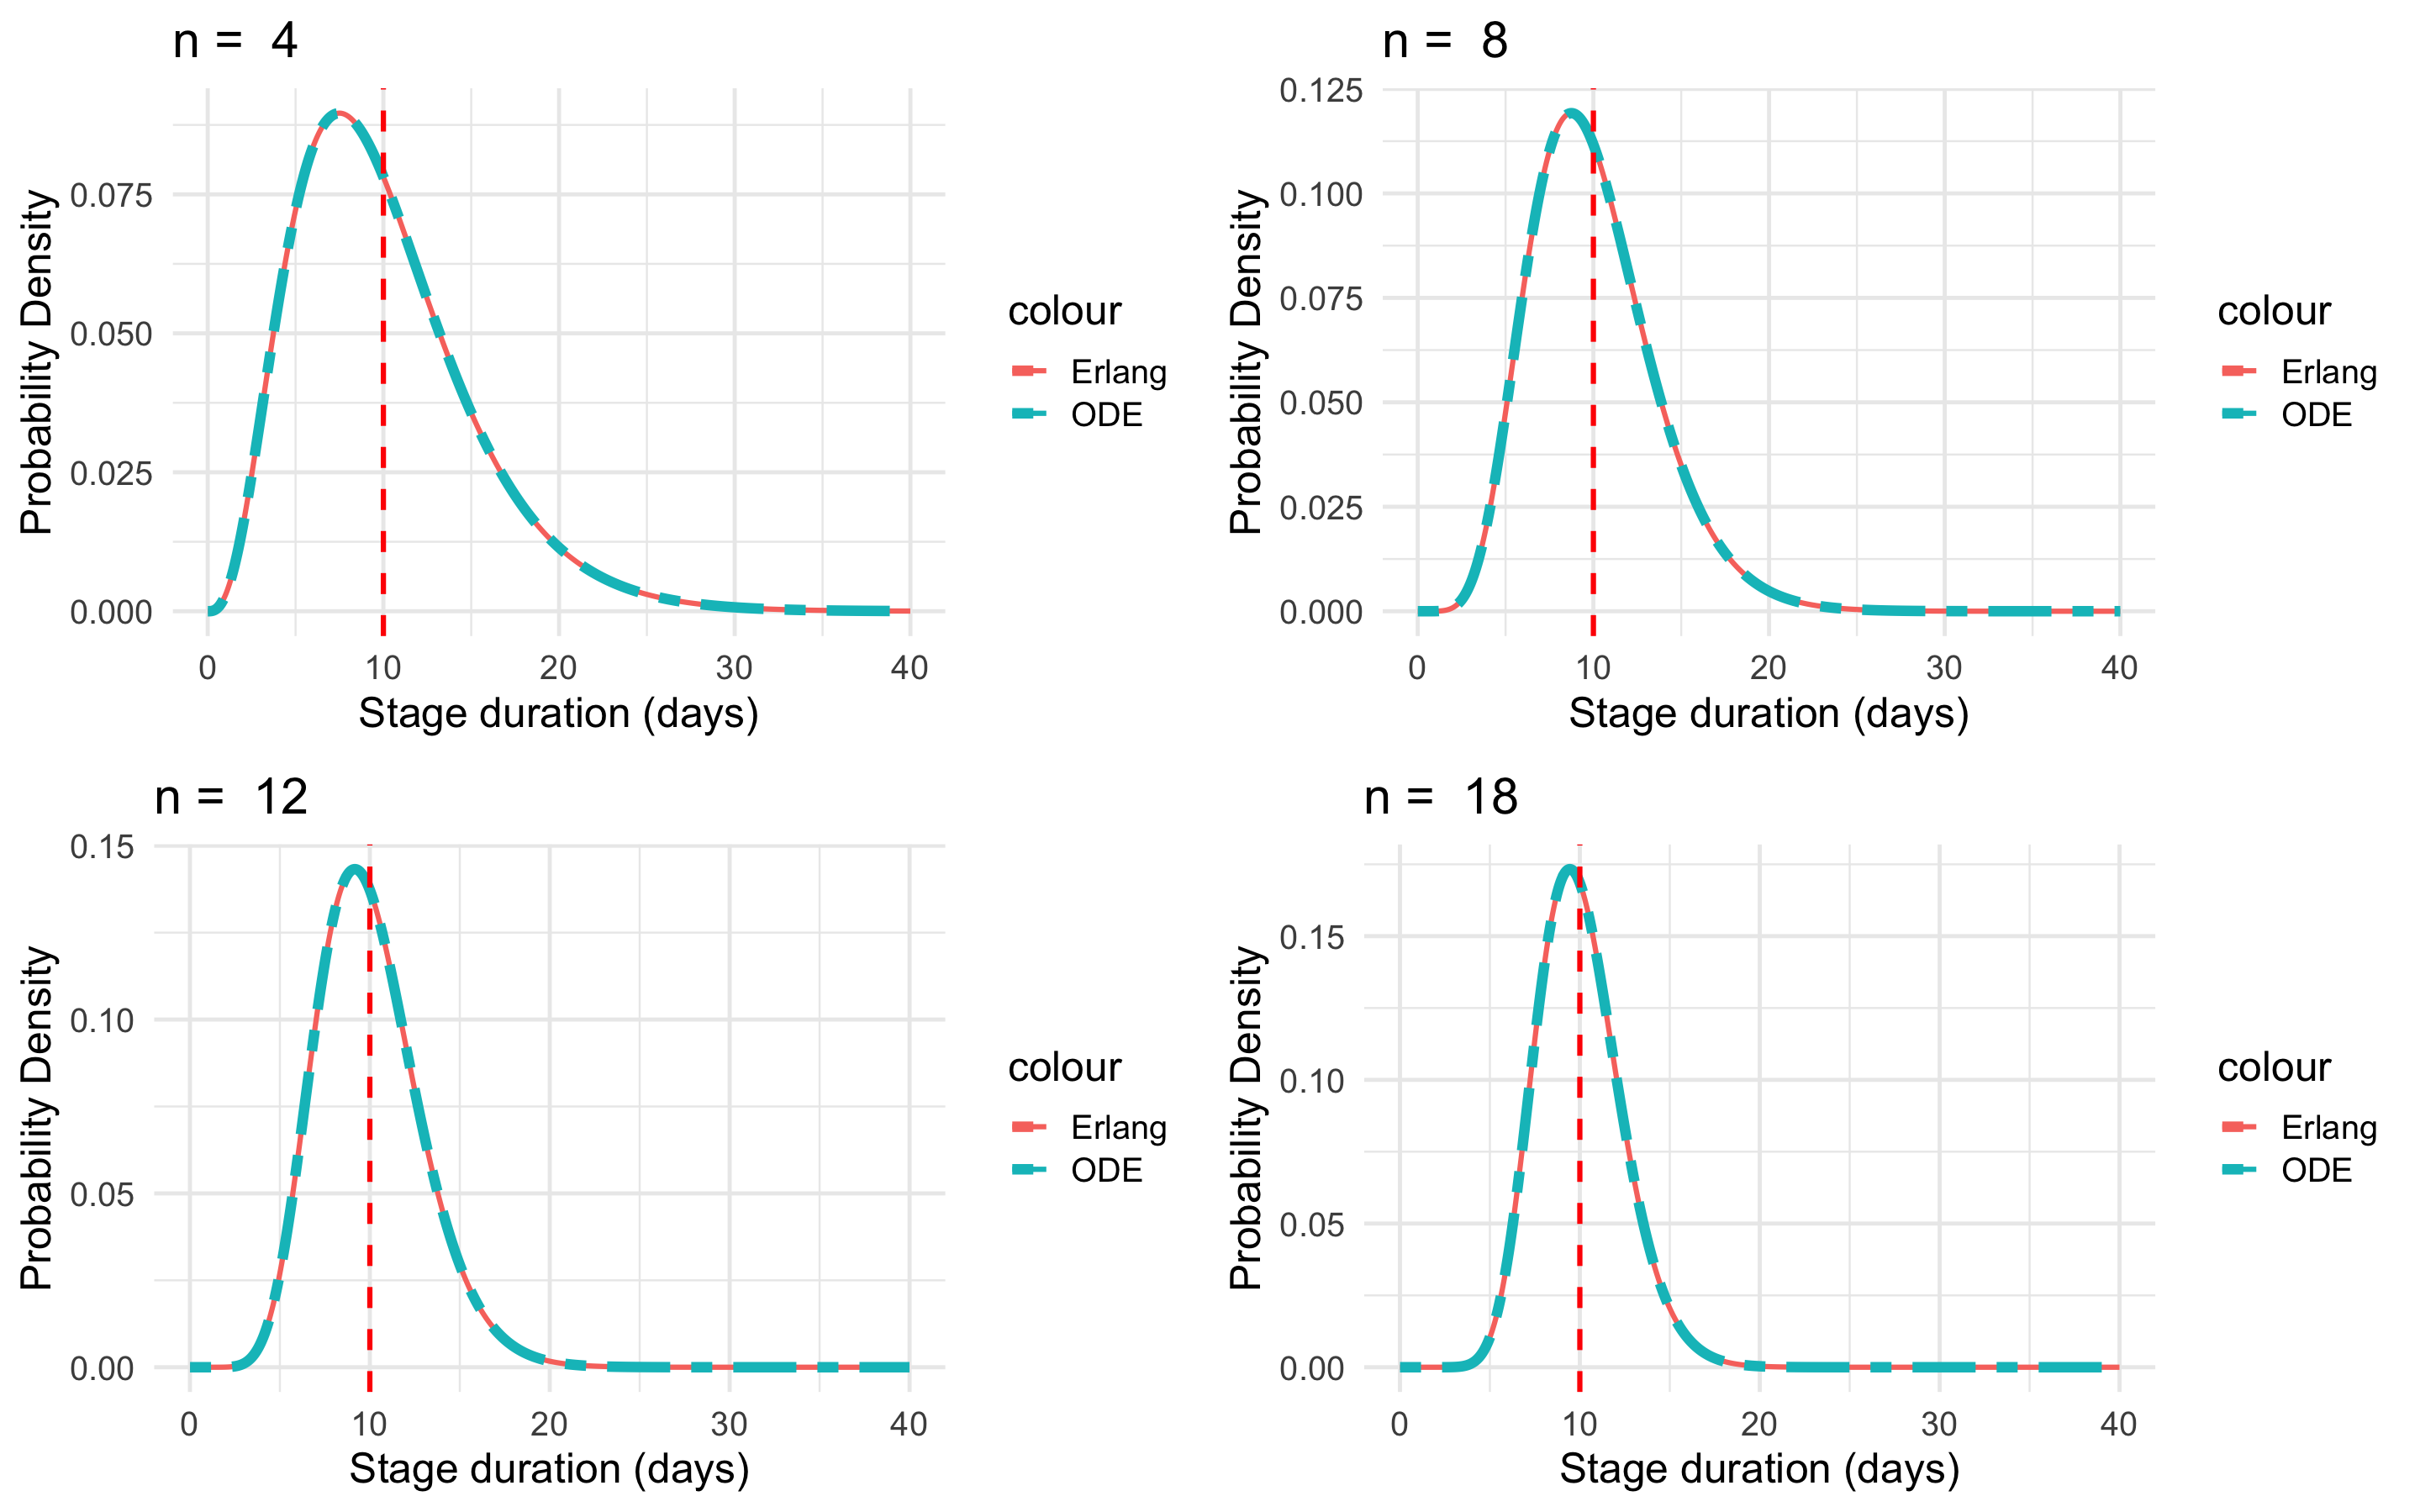
\includegraphics[width= 0.9\textwidth]{4.png}
    \caption{Probability Distribution Comparison Between Erlang and SI$^n$R Model}
\end{figure}
JD: Respect the units!

\subsection{Possible match between SI$^n$R and SIgR}
In the initial step following the successful construction of the SIgR model, which employs a fixed number of substages and a geometrically distributed substage rate, we want to evaluate the theoretical possibility of a match between the stage duration distribution produced by the SIgR model and that of the traditional SInR model. This match is defined in terms of two key parameters: the mean $(M)$ and the shape parameter $(\kappa)$.

The substage number of the SIgR model $(n_f)$ has been fixed at 12, and the mean stage duration for the entire infectious period is set to 10 days. We examine the effect of using 2, 4, and 8 infectious substages in the SI$^n$R model $(n = 2, 4, 8)$ on the values of $r$ required for the SIgR model to align formulaically with the shape parameter $(\kappa)$. In Figure 2, the plots on the left illustrate the changes in stage duration distribution in SIgR model resulting from varying $r$ within a range that includes the formulaic match for $\kappa$. The black curve represent duration distribution from the SI$^n$R model with the associated $n$. Plots on the right depict the variations in $\kappa$, calculated using the corresponding r values, where the red dashed line is the target value of $\kappa$. It is evident from the plots that, within the specified range of r, there is a concurrence in both the mean and shape parameter values between the SInR and SIgR model. These findings suggest that the results generated by the traditional mode are replicable using the model we propose.

\begin{figure}[h!]
    \centering
 
    \begin{subfigure}{0.6\linewidth}
       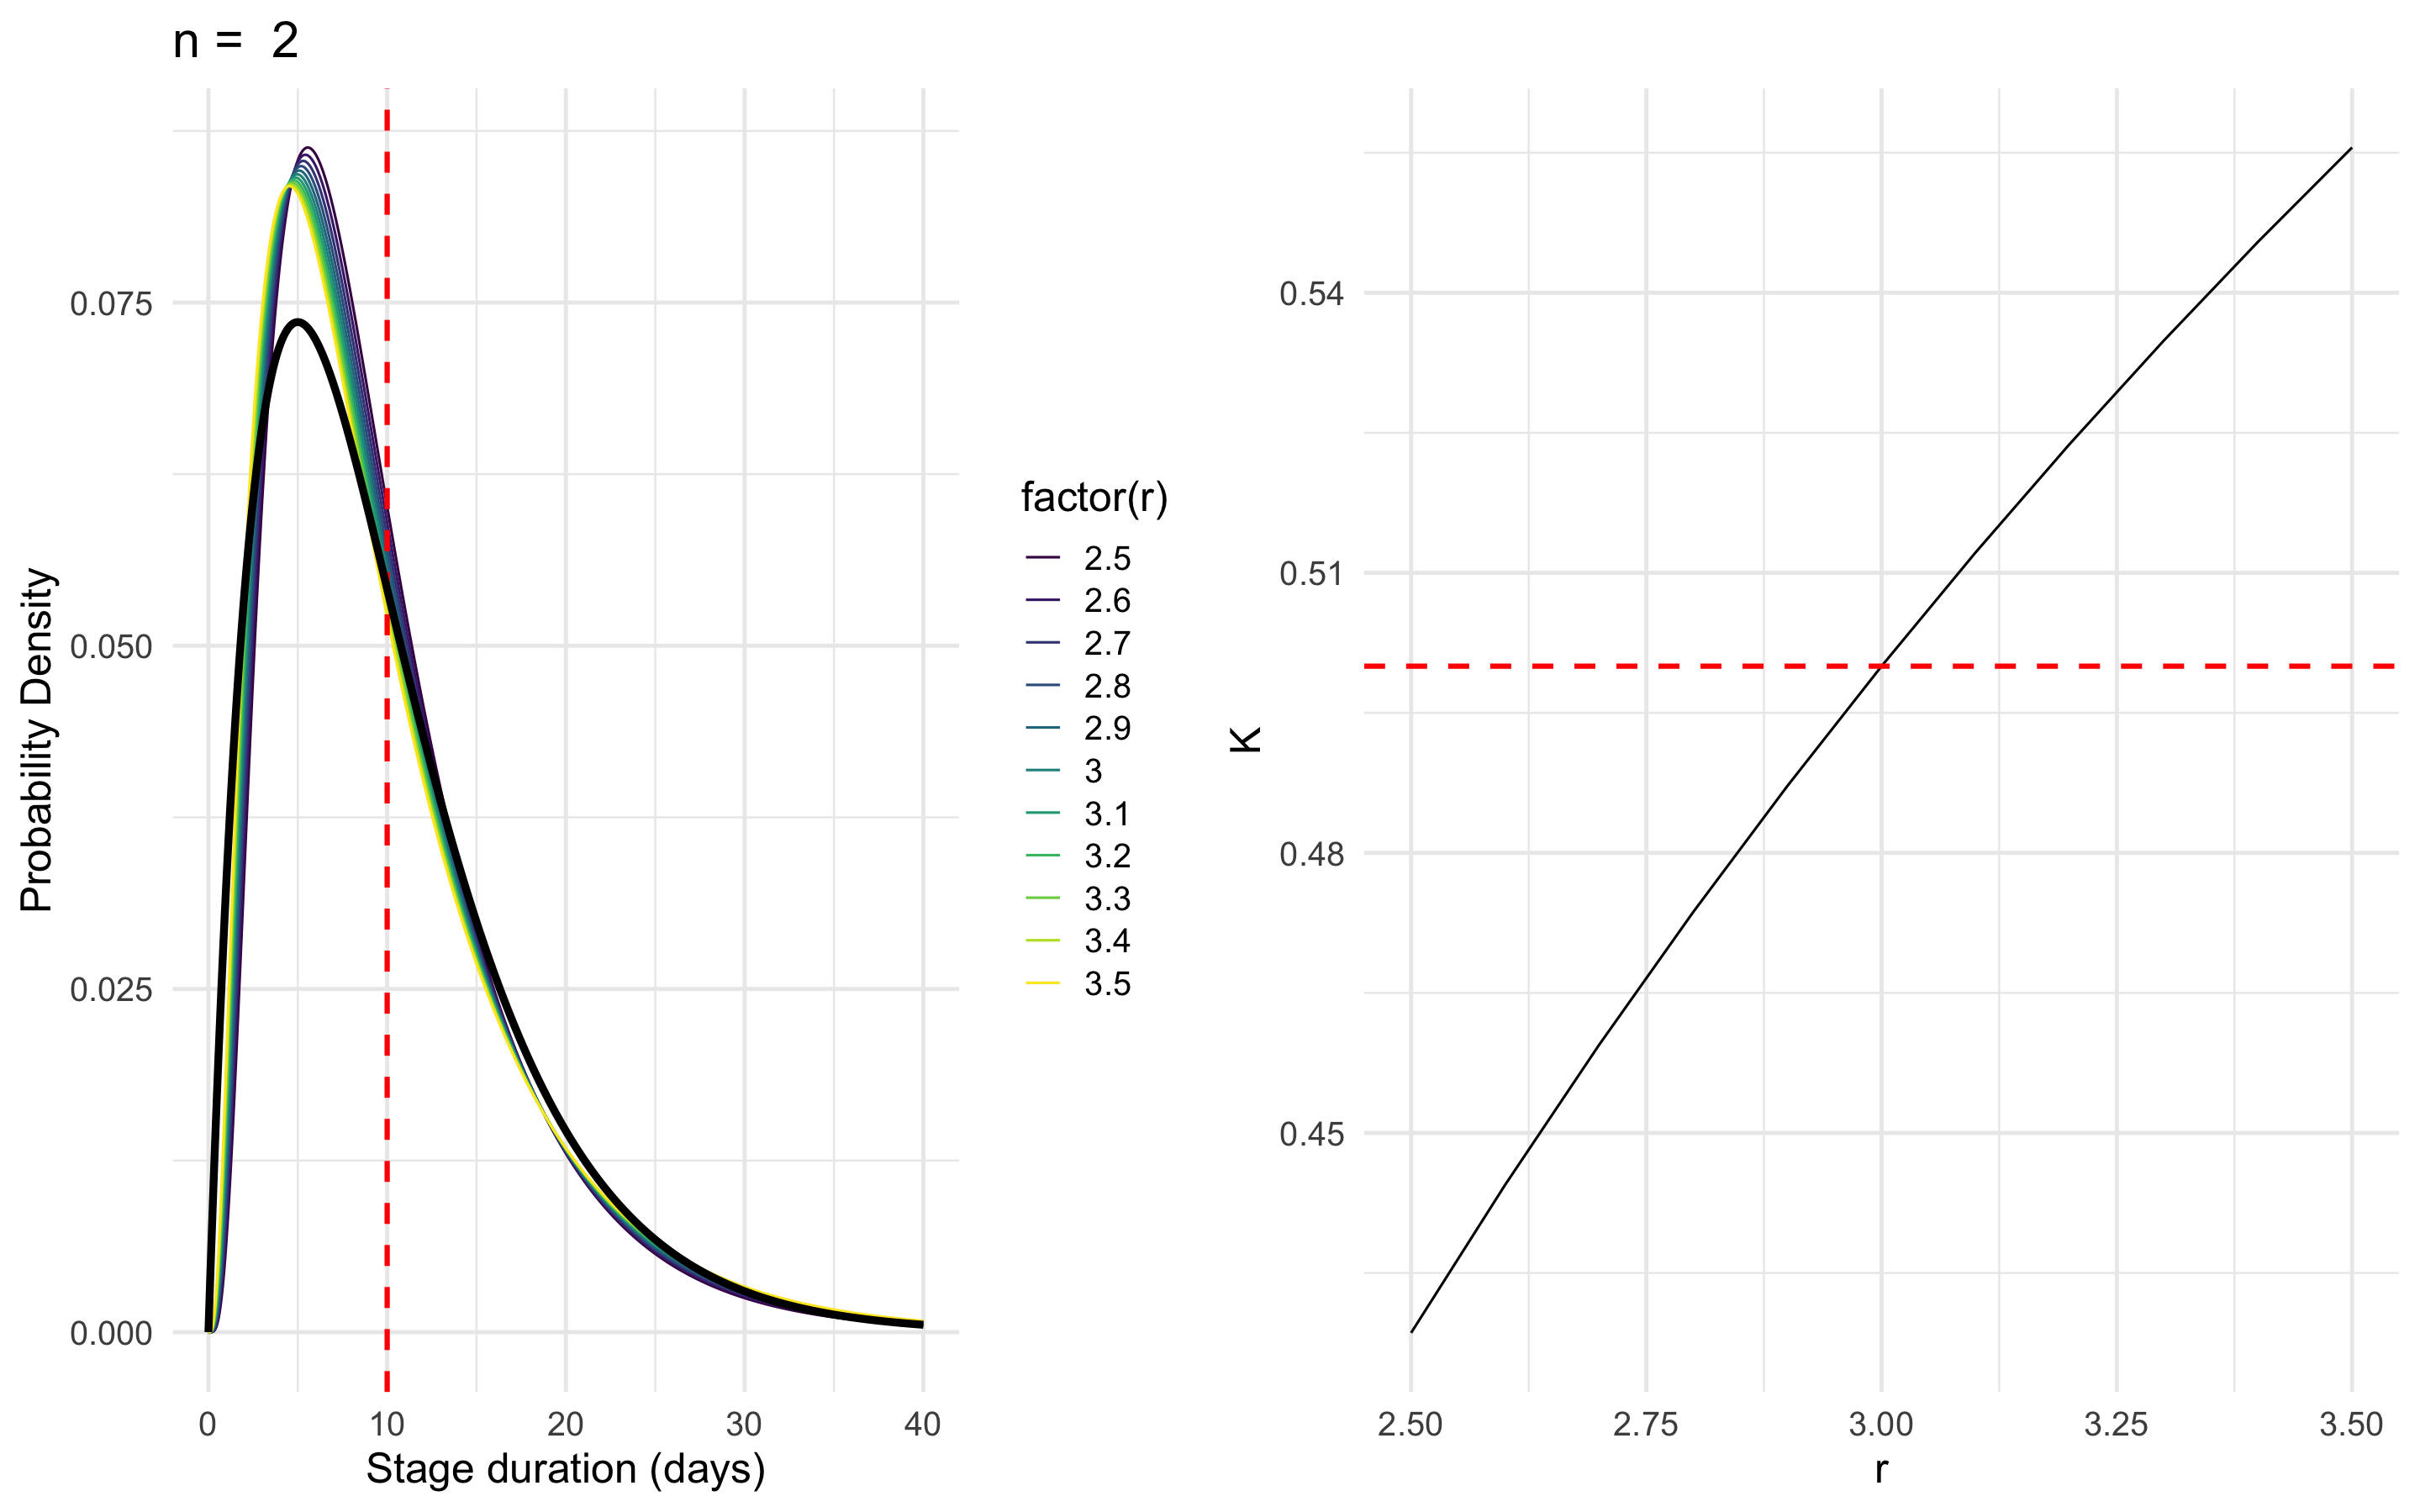
\includegraphics[width=\linewidth]{4.1(n=2).png}
    \end{subfigure}

    \begin{subfigure}{0.6\linewidth}
       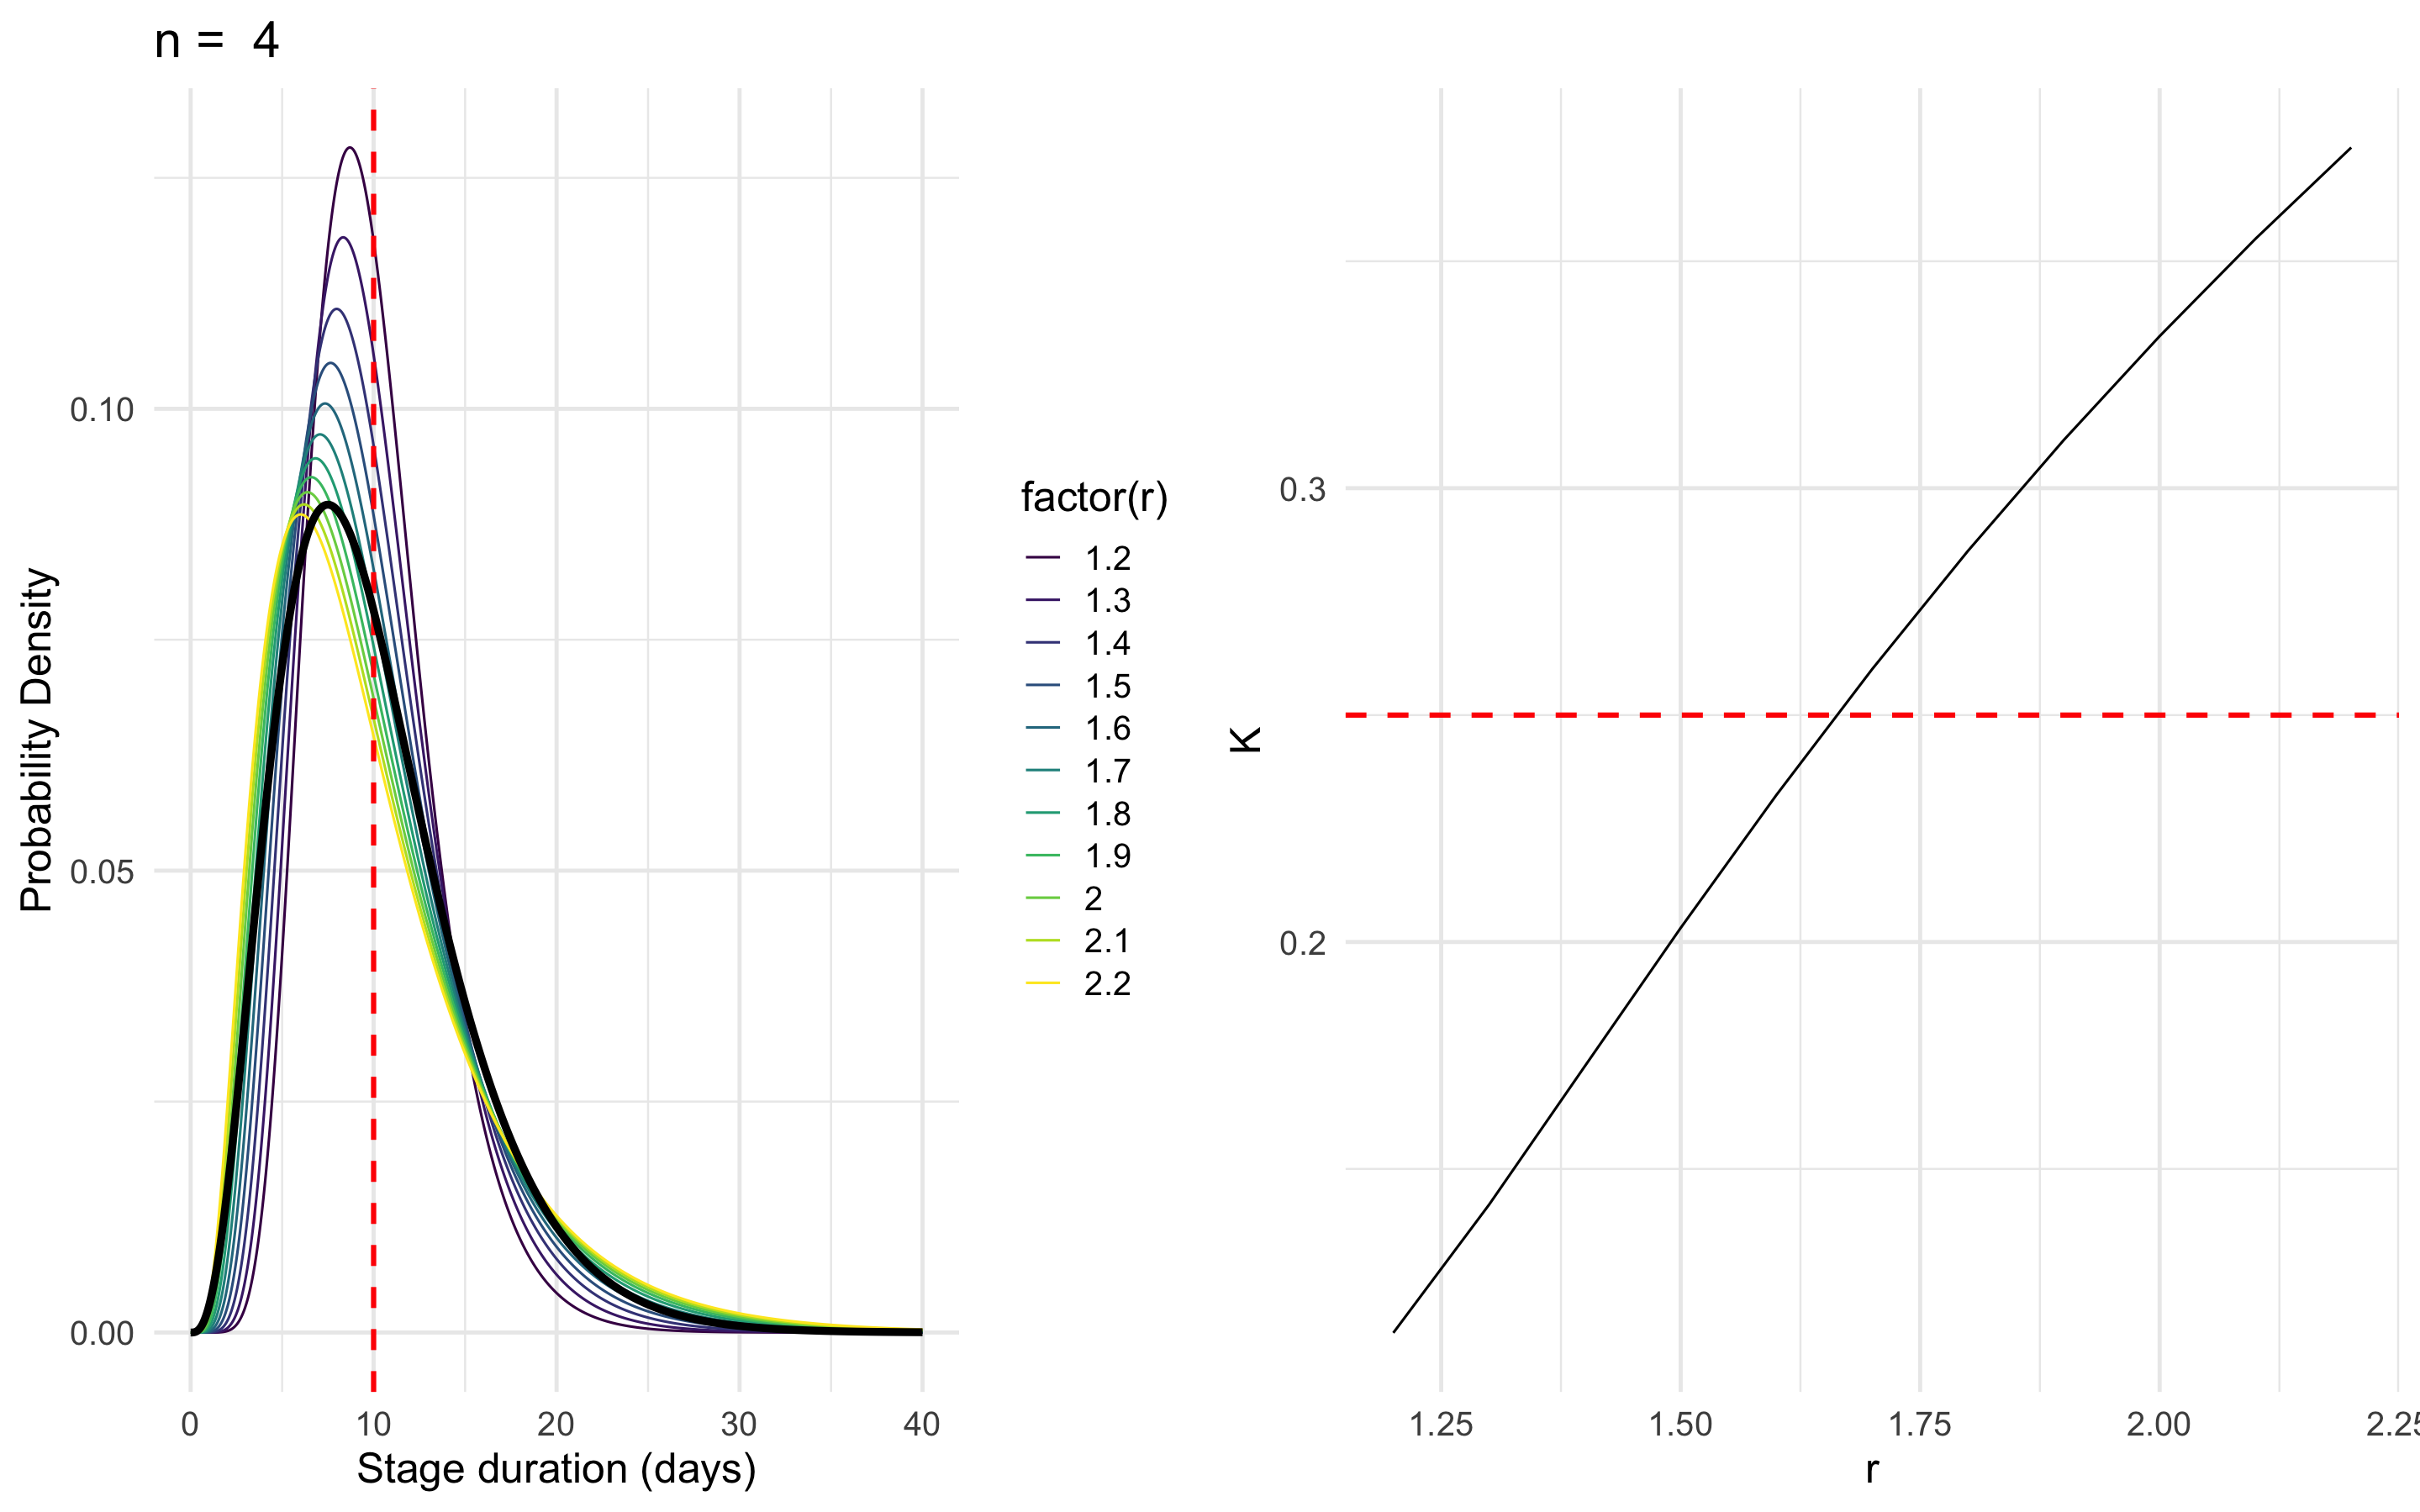
\includegraphics[width=\linewidth]{4.1(n=4).png}
    \end{subfigure}

    \begin{subfigure}{0.6\linewidth}
        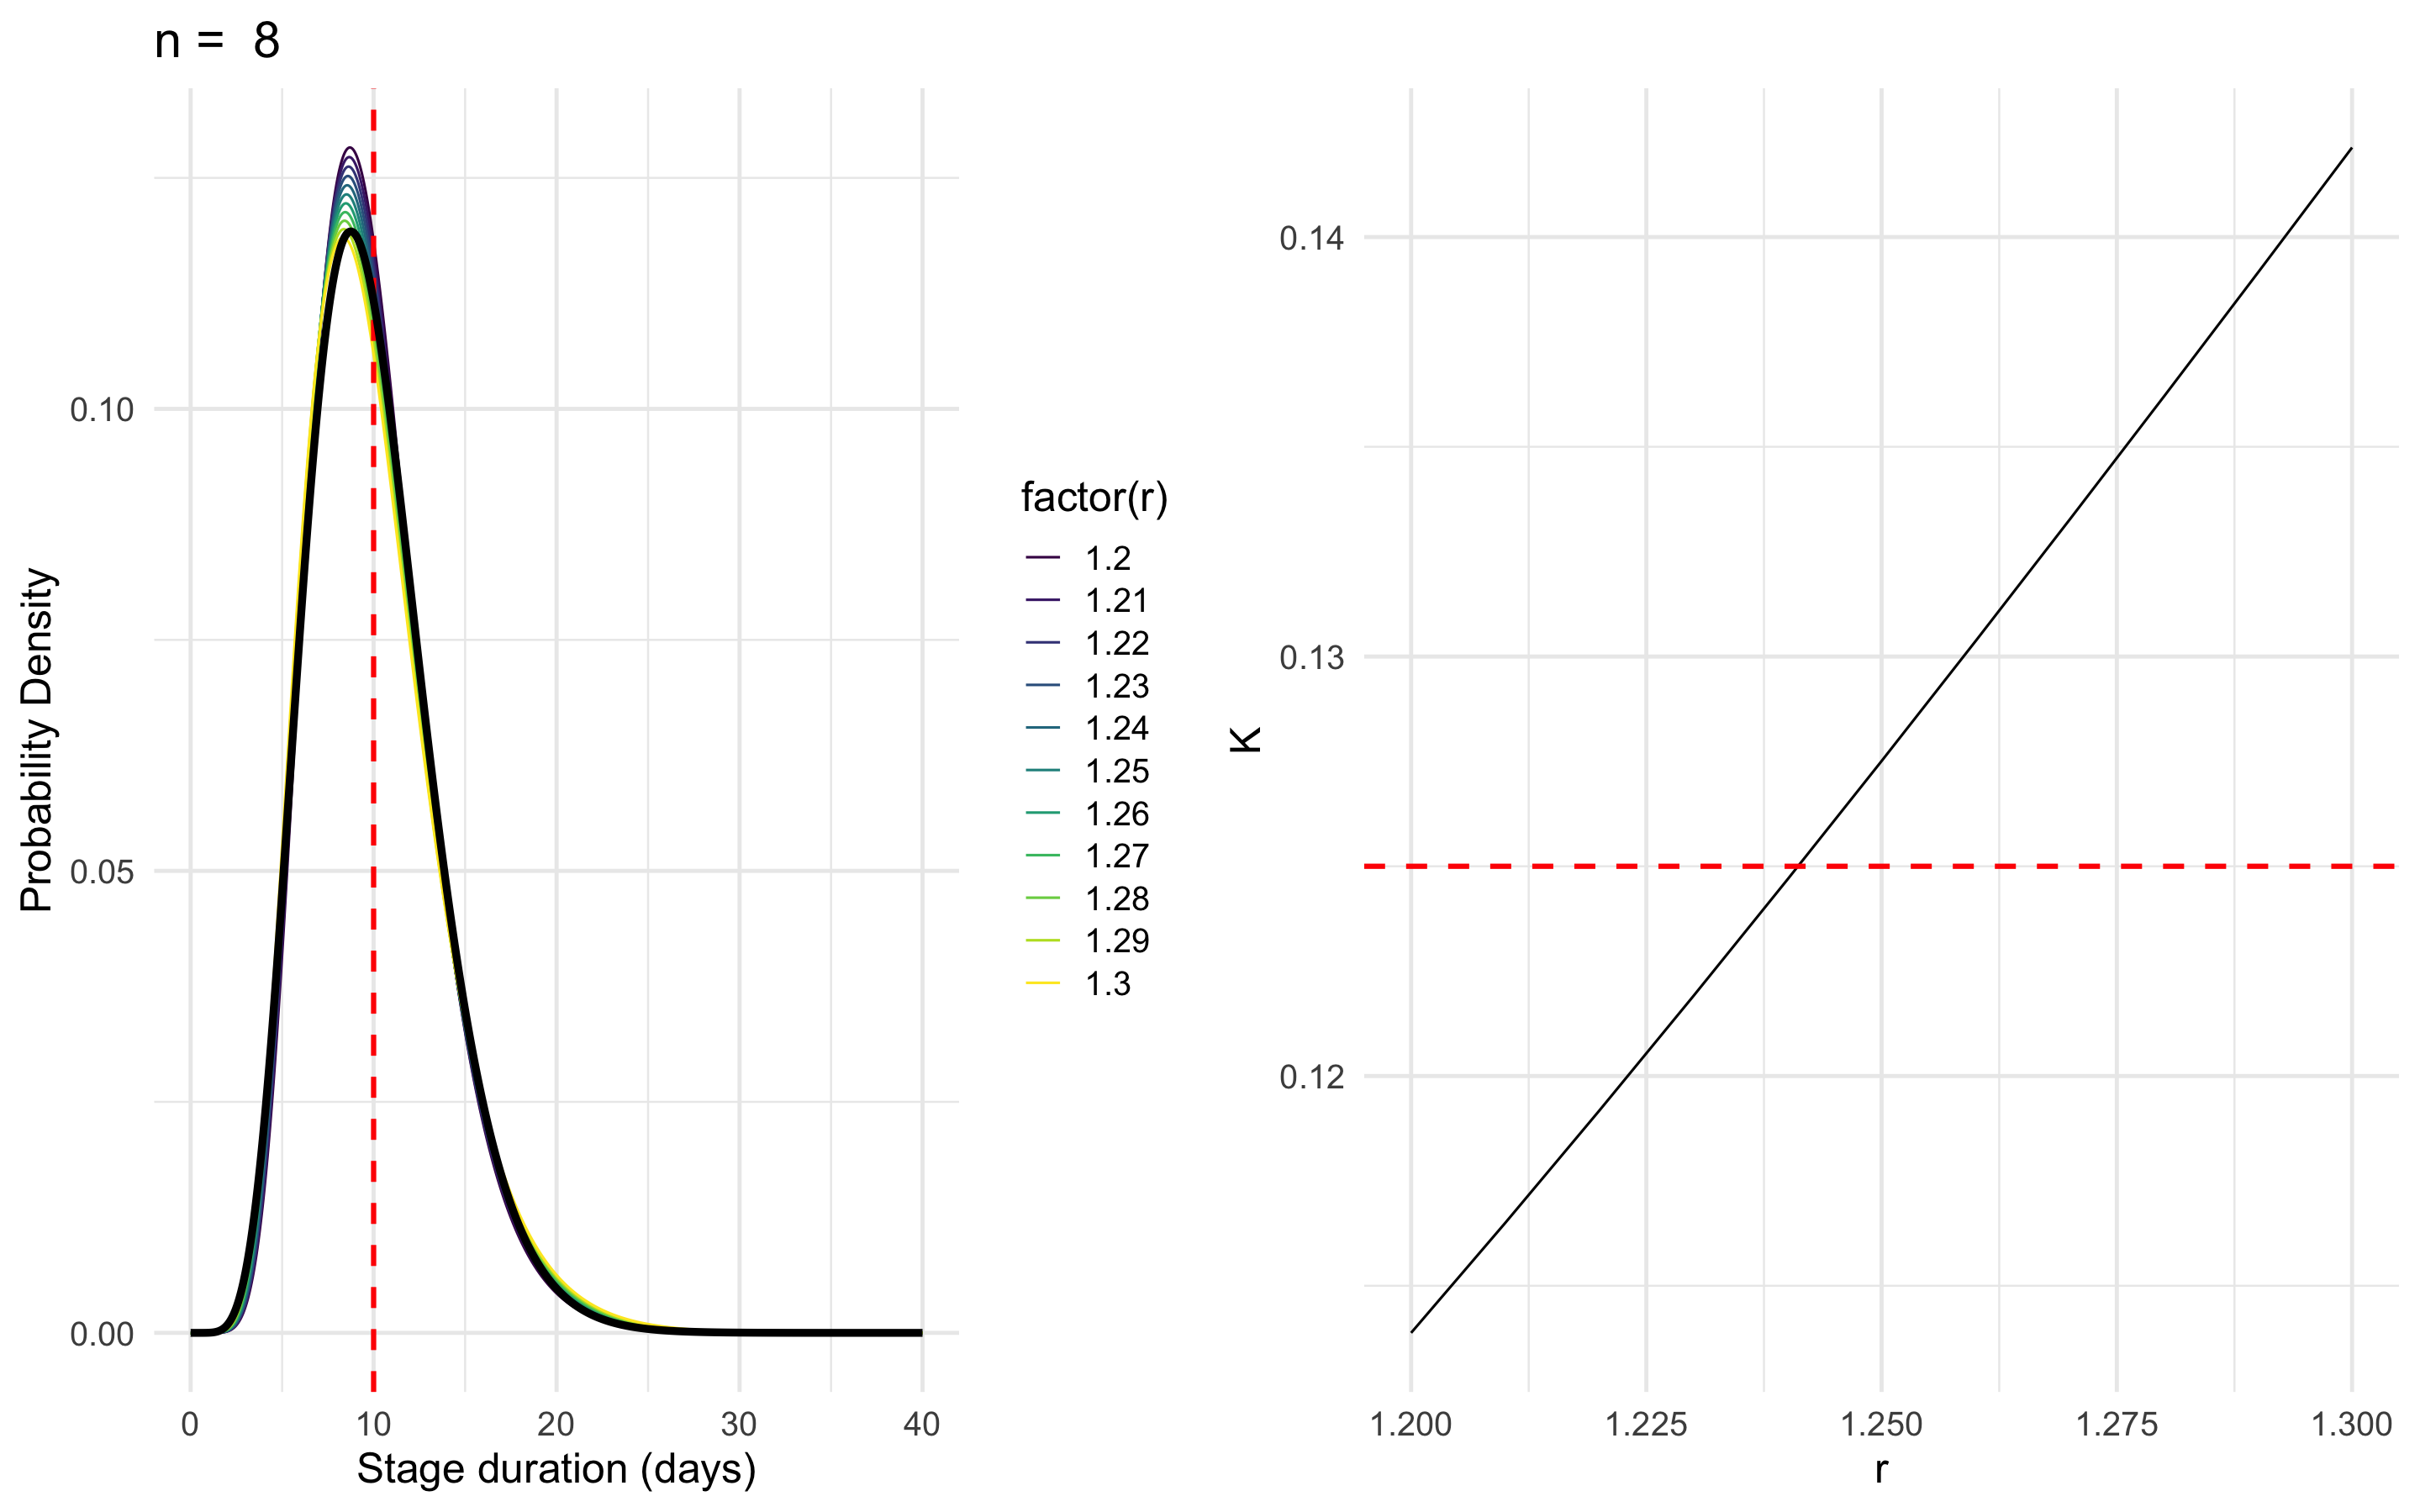
\includegraphics[width=\linewidth]{4.1(n=8).png}
     \end{subfigure}
 
    \caption{Adjusting $r$ to Evaluate Match While Preserving Mean Value}
    \label{fig:all_plots}
 \end{figure}
 

\subsection{Simple Equations Facilitating Independent and Flexible Changes in Mean and $\kappa$}
In the SIgR model, the calculation of the Mean $(M)$ and Variance $(\sigma^2)$ for the infectious stage duration distribution is accomplished by adding the corresponding properties of each substage, as follows:
\begin{align}
    Mean: \quad  &\sum_{i=1}^{n_f} \frac{1}{\gamma_i} = \frac{\frac{1}{a} (\frac{1}{r^n} - 1)}{\frac{1}{r} -1} \\
    Variance: \quad &\sum_{i=1}^{n_f} \left(\frac{1}{\gamma_i} \right)^2 = \frac{\frac{1}{a^2} (\frac{1}{r^{2n}} - 1)}{\frac{1}{r^2} -1}
\end{align}
The shape parameter $\kappa$, determined by $\frac{\sigma^2}{M}$, can thus be simplified to:
\begin{align}
    \kappa = \frac{(1+r^{n_f}) (1-r)}{(1+r) (1-r^{n_f})}
\end{align}
This simplification reveals that the value of $\kappa$ is exclusively dependent on the parameter $r$, thereby granting the model independence in property changes. This independence allows for the alignment of $\kappa$ without altering the Mean, achievable through adjustments to parameter $a$. Similarly, the Mean can be scaled to a desired value without impacting $\kappa$.

JD: I would frame this differently. Both PE and Erlang \emph{can} change the value of $n$; the real difference is that PE can be flexible even when $n$ doesn't change.
Importantly, it should be noted that the value of $\kappa$ is not affected by changes in the number of substages, as $n_f$ is fixed. Consequently, $\kappa$ can be any real number within the range $[\frac{1}{n_f}, 1)$, thereby significantly enhancing the model's flexibility. In contrast, in the SI$^n$R model, the value of $\kappa$ depends on how the substages are partitioned. Following the same steps of calculation, we obtain: $\kappa = \frac{1}{n}$. The shape parameter $\kappa$ in the SI$^n$R model is therefore restricted to a set of discrete values:
\begin{align*}
    \kappa \in \left\{1, \frac{1}{2}, \frac{1}{3}, \dots \right\}
\end{align*}
This limitation potentially reduces the capability of the SI$^n$R model to accurately reflect real-world scenarios.

\subsection{Identifying Parameters $a$ and $r$ to Align SI$^n$R and SIgR with Given Mean and $\kappa$}
Utilizing formulas (4) and (6), we have developed a computational system to reverse-engineer the process. The parameters $a$ and $r$, generated by this system, were reintegrated into the SIgR model. This enable us to compare the stage duration distribution with that of the SI$^n$R model, which possesses identical mean and shape parameters, as depicted in Figure 3. Although the formulaic $M$ and $\kappa$ are computed to be the same, we also conducted a numerical calculation of both properties, with results presented in Table 1. This analysis confirms that a match is achieved at both the formulaic and numerical levels. The visual discrepancies observed between the two distributions in Figure 3 can be considered negligible, since both distributions serve as theoretical representations of real-world scenarios and do not require exact correspondence.
\begin{figure}[h]
    \centering
    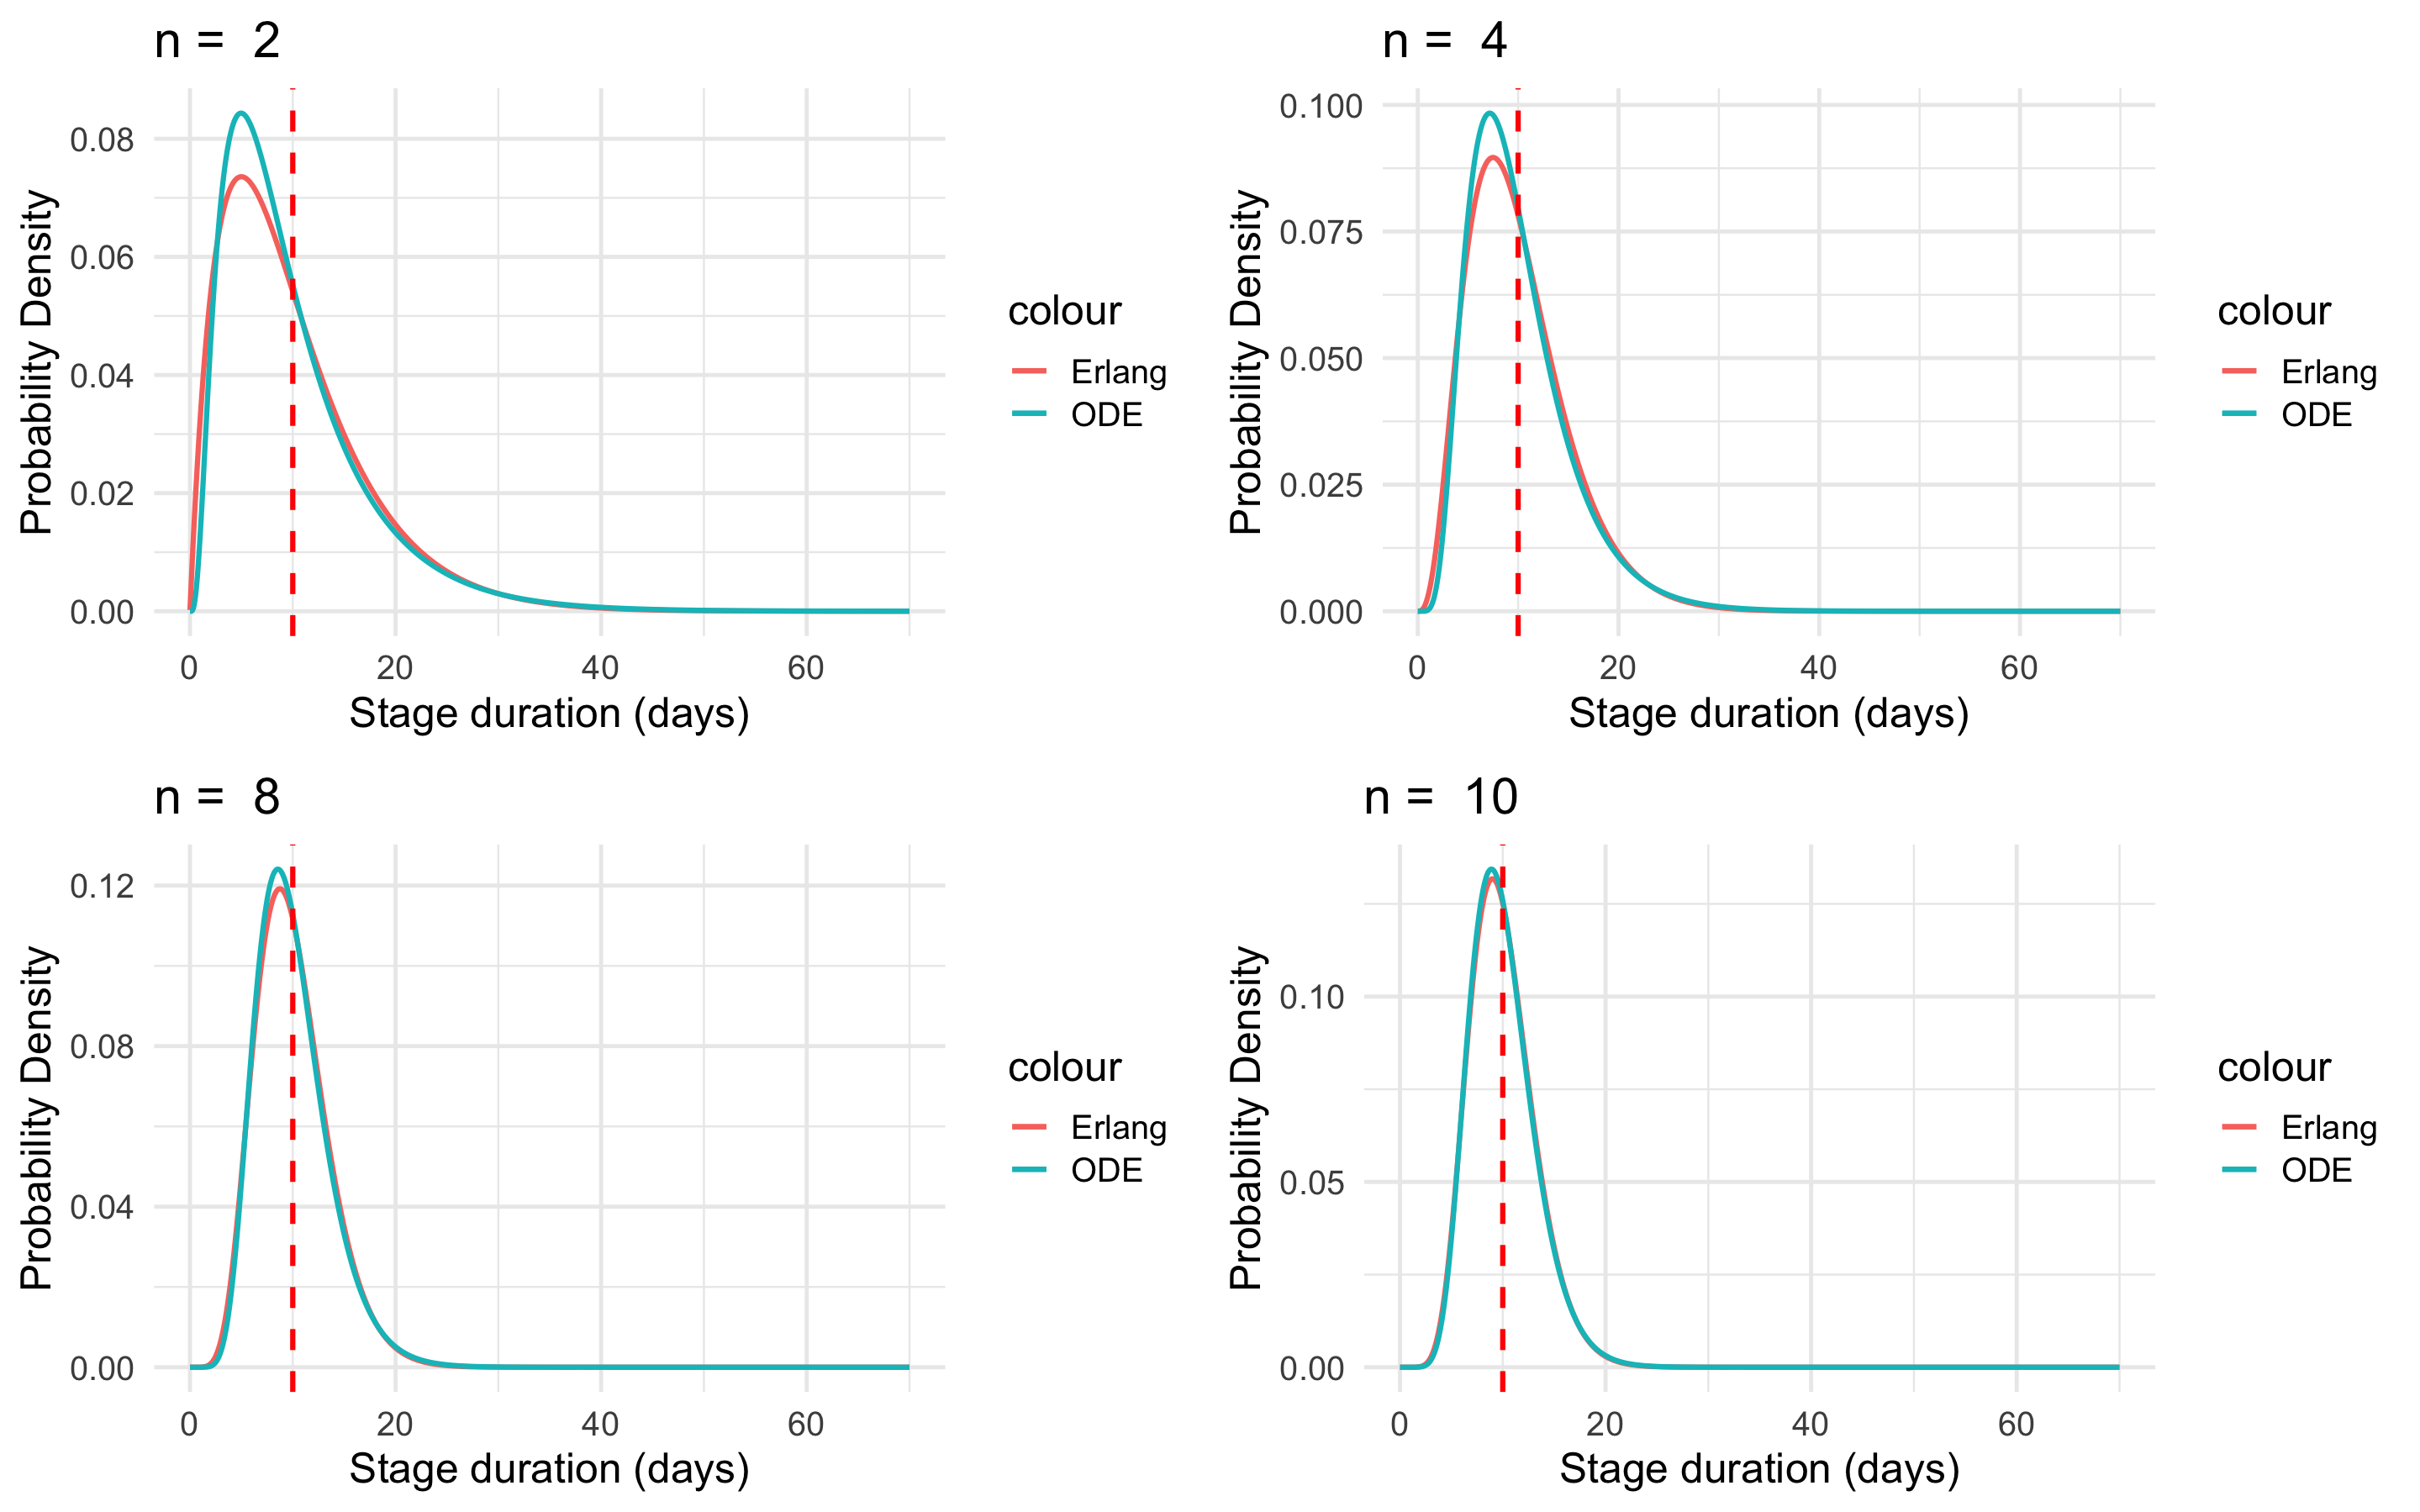
\includegraphics[width= \textwidth]{4.3.1.png}
    \caption{Theoretical Alignment of Mean and Shape Parameters in SI$^n$R and SIgR Models with Calculated Parameter Values $a$ and $r$}
\end{figure}

\begin{table}[h!]
    \centering
    \begin{tabular}{ l | c | r }
      \hline
      Substages & Mean & $\kappa$ \\
      \hline
      n = 2 & 10.000000 & 0.4999971 \\
      n = 4 & 10.000000 & 0.2500002 \\
      n = 8 & 10.000 & 0.125 \\
      n = 12 & 10.000000 & 0.0999986 \\
      \hline
    \end{tabular}
    \caption{Numerically Calculated Parameter Values From the SIgR Model}
\end{table}

JD: A table caption should have a clear explanation of what's in the table for people who are skimming (your figure captions should probably be improved, too). It's not clear what you're showing here, or whether it's right. Maybe show target values as well as observed values? Also, there seems to be a mismatch between $n=12$ and the corresponding $\kappa$? Also, there are too many significant figures here. We don't need to fix this table, since we don't need it moving forward, these are just general tips.

By incorporating the infectious stage duration distribution back into the entire SI$^n$R and SIgR models, we also present the dynamics of the infectious population density generated directly from the simulations. In Figure 4, using $n=2$ and $n=4$ for the SI$^n$R model and corresponding $a$ and $r$ values ( $r_2=2.9999604, a_2=0.1500007, r_4 = 1.6626998, a_4 = 0.2503359$) for the SIgR model, a close match is observed between the results generated by the two different methods. This indicates that the results of the SInR model are reproducible using the SIgR model, but with enhanced flexibility in parameter value changes.
\begin{figure}[h]
    \centering
    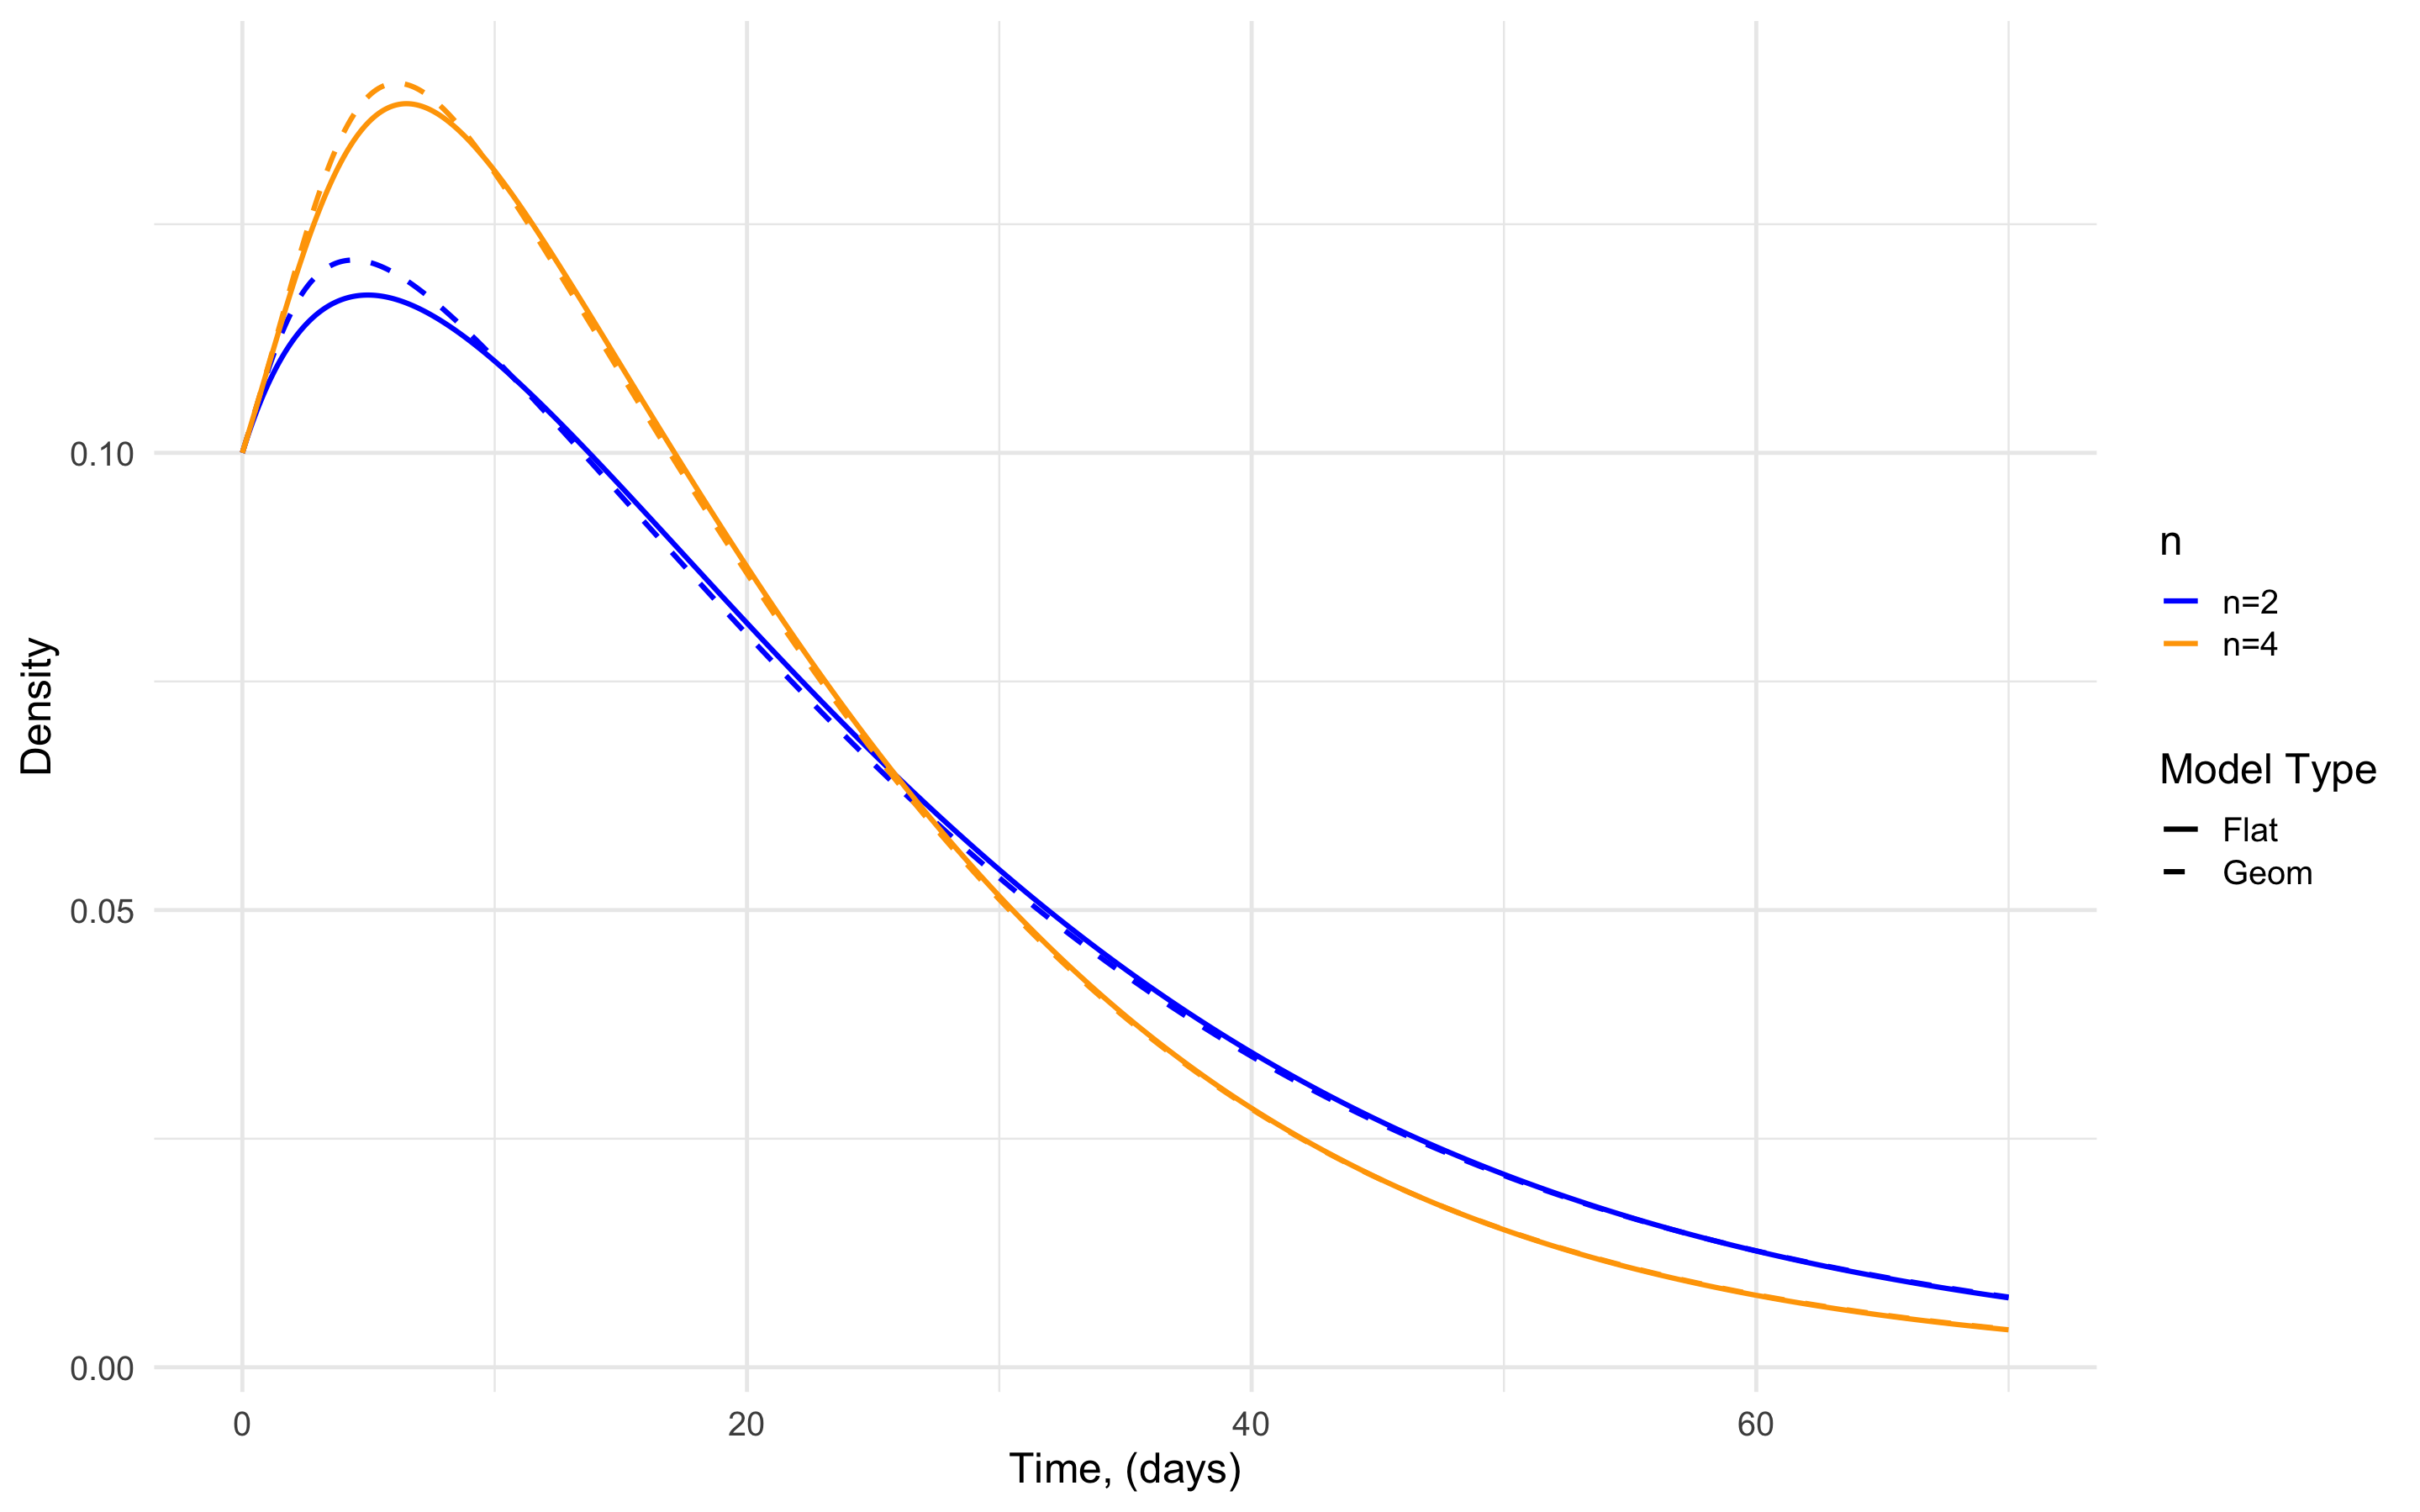
\includegraphics[width= \textwidth]{4.3.2.png}
    \caption{Simulation Comparison of the Population Dynamics Between SI$^n$R and SIgR Model with Equivalent Mean and Shape Parameter}
\end{figure}

\subsection{Enhanced Flexibility in Controlling Stage Duration Distribution Shapes}
Besides offering a simpler approach to constructing an epidemic model with efficacy comparable to the SInR model, the SIgR model further enhances our ability to manipulate the shape of the stage duration distribution. This is achieved by allowing the selection of any $\kappa$ value within the range $(\frac{1}{n_f}, 1)$. Figure 5 showcases the probability distribution plots generated by the SIgR model, given a desired mean $(M=10)$ and selected $\kappa$ value $(\kappa = 0.25, 0.45, 0.65, 0.85)$. This chosen $\kappa$ value (except 0.25) is unattainable in the SI$^n$R model, distinguishing the SIgR model's unique capabilities. The new model adeptly incorporates a wider array of distribution shapes into the SIR framework. It emerges as a versatile tool for capturing a more extensive range of dynamic patterns in disease spread and control.
\begin{figure}[h]
    \centering
    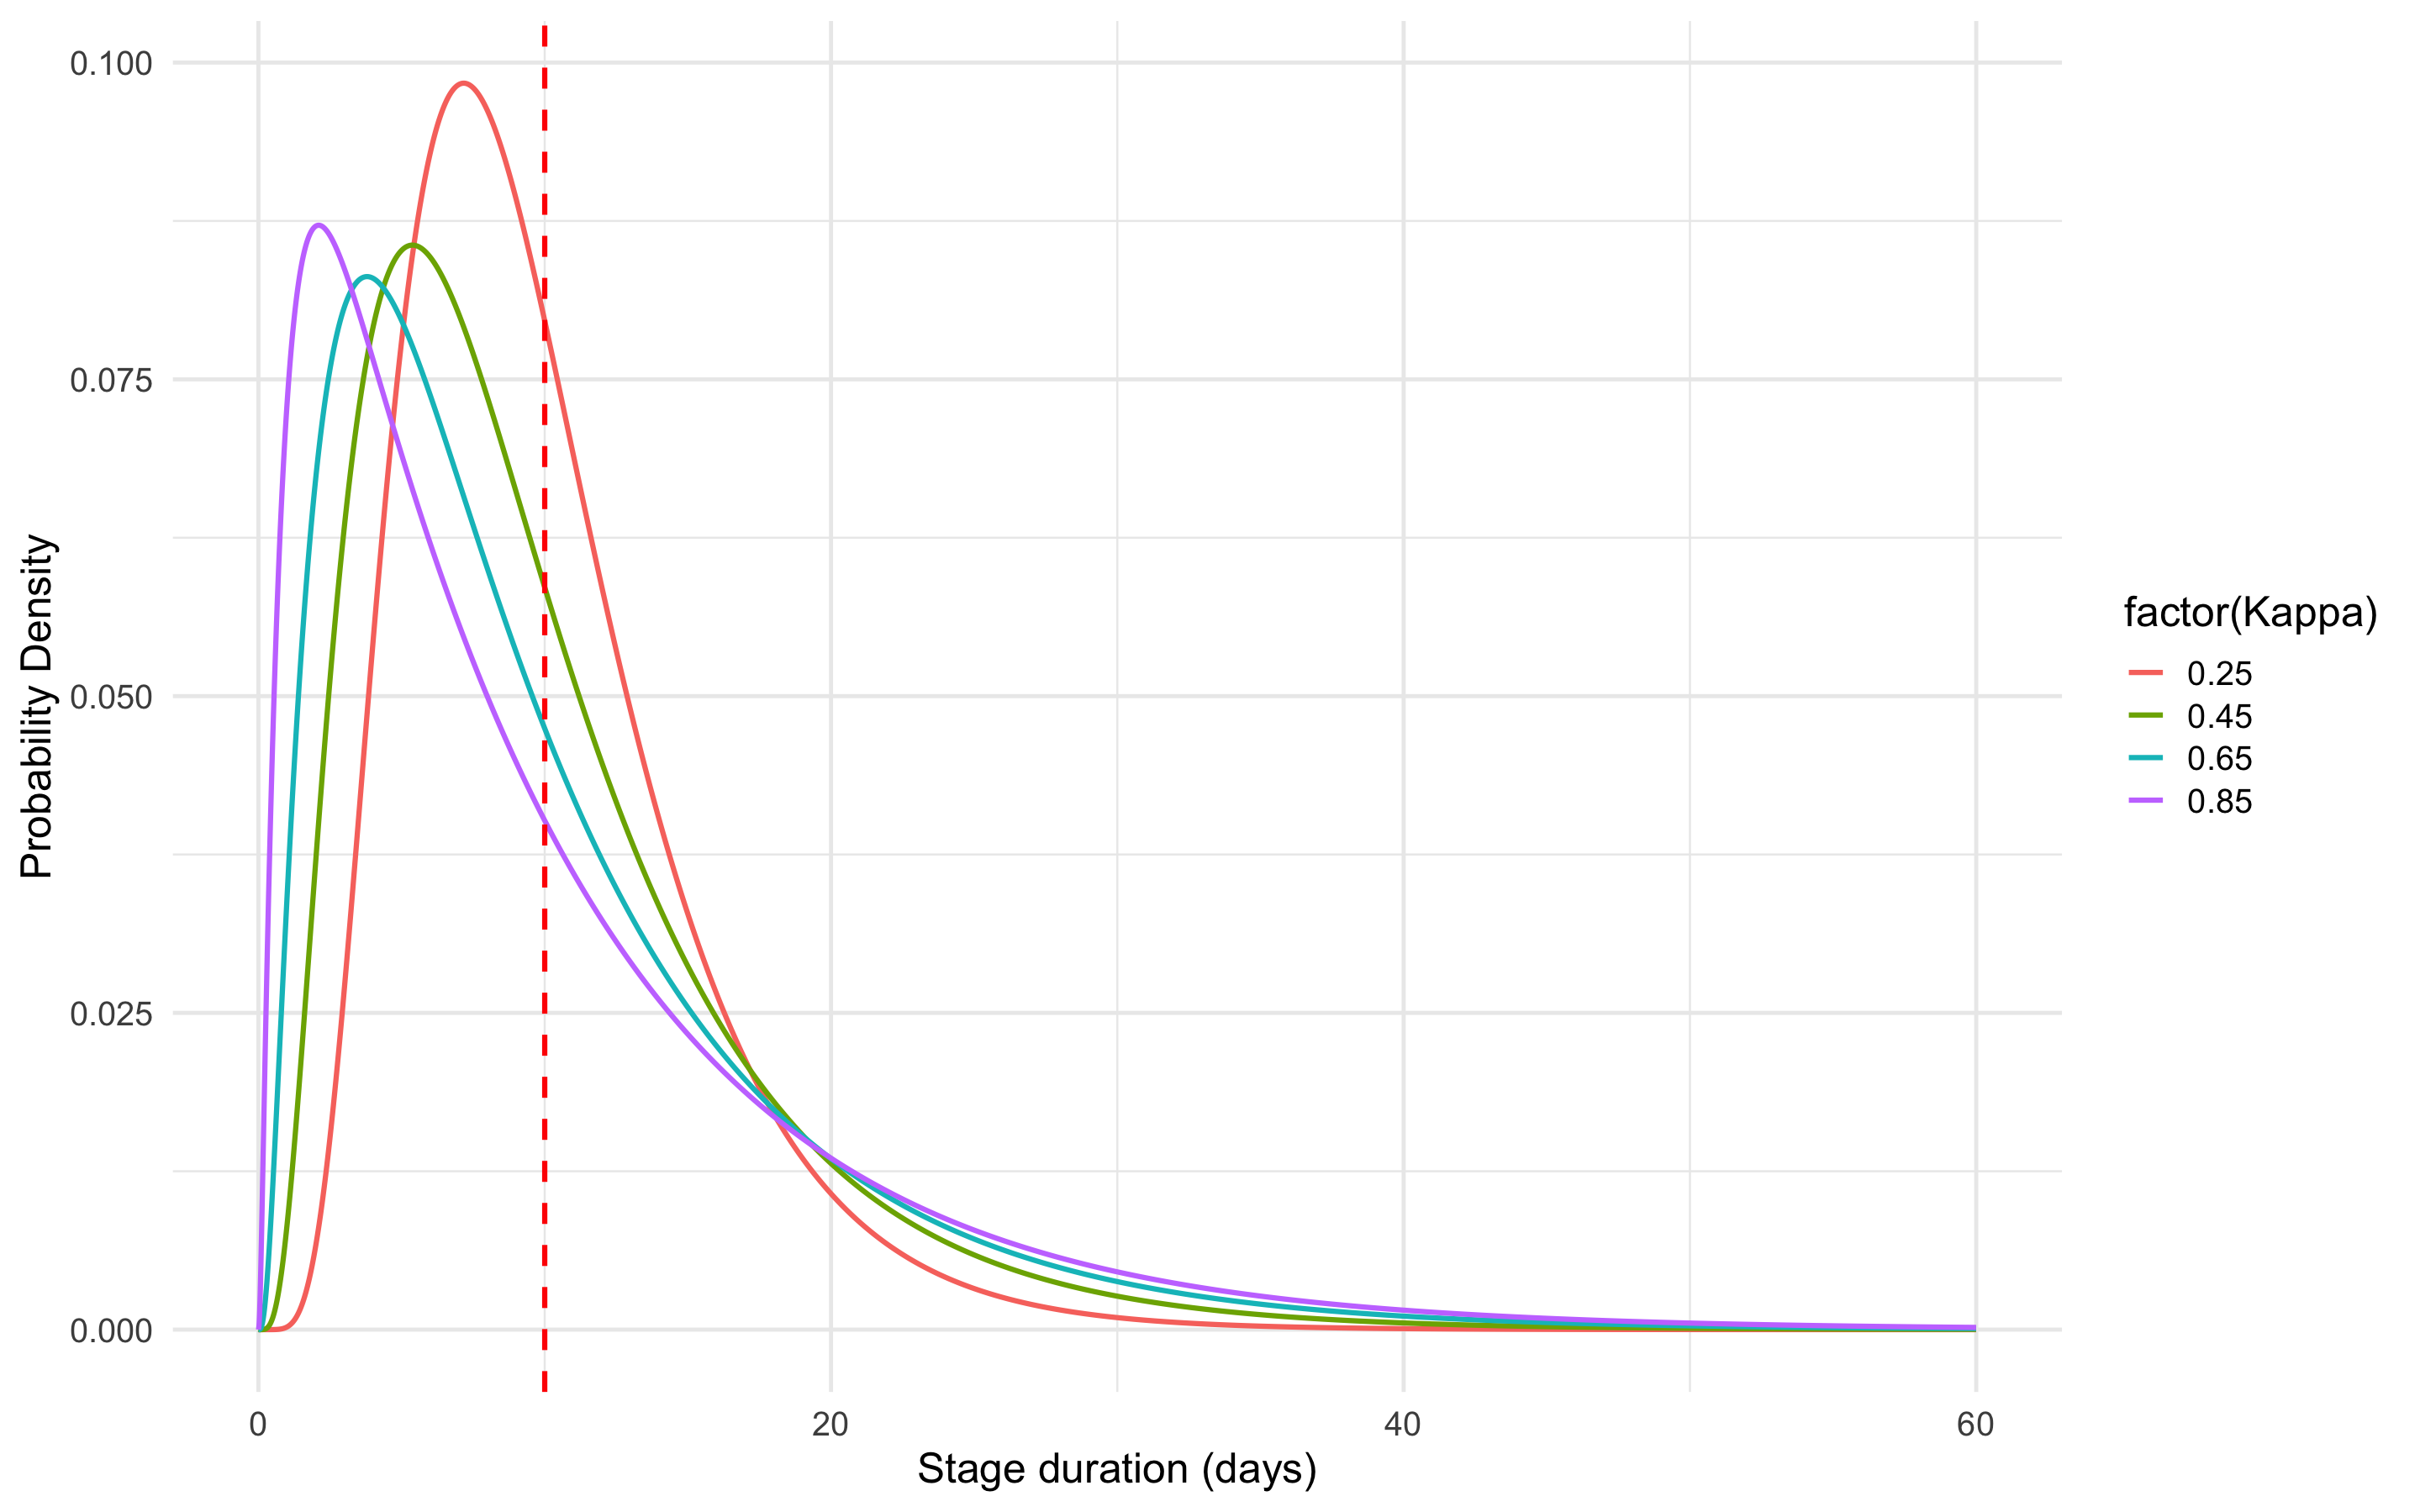
\includegraphics[width= \textwidth]{4.4.2.png}
    \caption{Generating Stage Duration Distributions with Custom Mean and Shape Parameters Using the SIgR Model}
\end{figure}

    


\section{Discussion}
SIR compartmental models are widely utilized in modeling infectious diseases, but they encounter a significant limitation: the implicit assumption that the time an individual spends in the disease stage follows an exponential distribution. To address this issue, a common method involves subdividing the infectious stage into $n$ number of substages, each substage is exponentially distributed with a constant rate. This approach is also known as the Linear Chain Trick (LCT). LCT strategy facilitates an Erlang-shaped stage duration distribution with increased reality. However, this model also faces limitations, including cumbersome parameter optimization processes and the constraint of discrete parameter values, which can affect its performance.

In this study, we propose the SIgR model, which features a fixed number of infectious substages and a geometric distribution rate for these substages, as an alternative to the SInR model that incorporates LCT. In the results section above, we demonstrated that adjusting the parameters for the geometric series $a$ and $r$ allows us to replicate the simulation results generated by the SInR model. Moreover, our model offers enhanced flexibility in shaping the distribution of the infectious stage duration, as it allows for the selection of mean $(M)$ and shape parameters $(\kappa)$ of the distribution such that $M \in \mathbb{R}^+$ and $\kappa \in [\frac{1}{n}, 1)$. Additionally, the fixed structure of our model simplifies the process of finding optimized parameter values, requiring only a one-time process during data fitting. This simplification streamlines the development of computer code for use with ODE solvers in R, ultimately saving time and reducing complexity.

Future work will primarily focus on fitting data to the model we have proposed. This will include both synthetic data generated through simulation and actual real-world data. The results of this fitting process will be compared with those obtained from the SInR model. Later on, we plan to incorporate process error considerations to increase the robustness of our model.

The anticipated outcome of this research is the development of a model that not only exceeds current models in terms of predictive accuracy but also maintains simplicity in implementation. The core design of our model is intended to be easily adaptable across various state transition models. This adaptability is vital for its application in diverse domains, ranging from epidemiology to system dynamics. The idea is designed to be extensible, capable of accommodating a range of distribution types and parameter sets. Such versatility makes it a powerful tool for modeling a wide array of complex systems, with the capability to adjust and evolve in response to new data and insights.

In conclusion, this study suggests that our method could simplify and enhance the fitting of models with flexible time distributions within an Ordinary Differential Equation (ODE) framework. This research has the potential to enhance model performance and to develop user-friendly tools for effective epidemic modeling and prediction.



\bibliographystyle{unsrt}
\bibliography{Reference} 

\end{document}
